%Version 3.1 December 2024
% See section 11 of the User Manual for version history
%
%%%%%%%%%%%%%%%%%%%%%%%%%%%%%%%%%%%%%%%%%%%%%%%%%%%%%%%%%%%%%%%%%%%%%%
%%                                                                 %%
%% Please do not use \input{...} to include other tex files.       %%
%% Submit your LaTeX manuscript as one .tex document.              %%
%%                                                                 %%
%% All additional figures and files should be attached             %%
%% separately and not embedded in the \TeX\ document itself.       %%
%%                                                                 %%
%%%%%%%%%%%%%%%%%%%%%%%%%%%%%%%%%%%%%%%%%%%%%%%%%%%%%%%%%%%%%%%%%%%%%

%%\documentclass[referee,sn-basic]{sn-jnl}% referee option is meant for double line spacing

%%=======================================================%%
%% to print line numbers in the margin use lineno option %%
%%=======================================================%%

%%\documentclass[lineno,pdflatex,sn-basic]{sn-jnl}% Basic Springer Nature Reference Style/Chemistry Reference Style

%%=========================================================================================%%
%% the documentclass is set to pdflatex as default. You can delete it if not appropriate.  %%
%%=========================================================================================%%

%%\documentclass[sn-basic]{sn-jnl}% Basic Springer Nature Reference Style/Chemistry Reference Style

%%Note: the following reference styles support Namedate and Numbered referencing. By default the style follows the most common style. To switch between the options you can add or remove “Numbered” in the optional parenthesis. 
%%The option is available for: sn-basic.bst, sn-chicago.bst%  
 
%%\documentclass[pdflatex,sn-nature]{sn-jnl}% Style for submissions to Nature Portfolio journals
%%\documentclass[pdflatex,sn-basic]{sn-jnl}% Basic Springer Nature Reference Style/Chemistry Reference Style
\documentclass[pdflatex,sn-mathphys-num]{sn-jnl}% Math and Physical Sciences Numbered Reference Style
%%\documentclass[pdflatex,sn-mathphys-ay]{sn-jnl}% Math and Physical Sciences Author Year Reference Style
%%\documentclass[pdflatex,sn-aps]{sn-jnl}% American Physical Society (APS) Reference Style
%%\documentclass[pdflatex,sn-vancouver-num]{sn-jnl}% Vancouver Numbered Reference Style
%%\documentclass[pdflatex,sn-vancouver-ay]{sn-jnl}% Vancouver Author Year Reference Style
%%\documentclass[pdflatex,sn-apa]{sn-jnl}% APA Reference Style
%%\documentclass[pdflatex,sn-chicago]{sn-jnl}% Chicago-based Humanities Reference Style

%%%% Standard Packages
%%<additional latex packages if required can be included here>
\let\labelindent\relax

\usepackage{etex}
\usepackage{amssymb,amsfonts,amsmath,amsthm}
\usepackage{graphicx}
\usepackage[usenames,x11names, dvipsnames, svgnames]{xcolor}
%\usepackage{amsmath,amssymb,amsthm}
\usepackage{dsfont}
\usepackage{amsfonts}
\usepackage{mathrsfs}
\usepackage{texshade}
\usepackage{hyperref}
\hypersetup{
  colorlinks=true,
  linkcolor=black,
  citecolor=blue,
  filecolor=black,
  urlcolor=DodgerBlue4,
  breaklinks=false,
  % linkbordercolor=red,% hyperlink borders will be red
  % pdfborderstyle={/S/U/W 1}% border style will be underline of width 1pt
}
\usepackage{tikz}
\usepackage{pgfplots}
\usepackage{tikzviolinplots}
\usetikzlibrary{shapes,calc,shadows,fadings,arrows,decorations.pathreplacing,automata,positioning}
\usetikzlibrary{external}
\usetikzlibrary{decorations.text}
\tikzexternalize[prefix=./Figures/External/]% activate externalization!
\tikzexternaldisable
\usetikzlibrary{patterns}
\usetikzlibrary{decorations.markings}
\usepackage{mathtools}
\usepackage[group-separator={,}]{siunitx}
%% ## Equation Space Control---------------------------
\def\EQSP{3pt}
\newcommand{\mltlne}[2][\EQSP]{\begingroup\setlength\abovedisplayskip{#1}\setlength\belowdisplayskip{#1}\begin{equation}\begin{multlined} #2 \end{multlined}\end{equation}\endgroup\noindent}
\newcommand{\cgather}[2][\EQSP]{\begingroup\setlength\abovedisplayskip{#1}\setlength\belowdisplayskip{#1}\begin{gather} #2 \end{gather}\endgroup\noindent}
\newcommand{\cgathers}[2][\EQSP]{\begingroup\setlength\abovedisplayskip{#1}\setlength\belowdisplayskip{#1}\begin{gather*} #2 \end{gather*}\endgroup\noindent}
\newcommand{\calign}[2][\EQSP]{\begingroup\setlength\abovedisplayskip{#1}\setlength\belowdisplayskip{#1}\begin{align} #2 \end{align}\endgroup\noindent}
\newcommand{\caligns}[2][\EQSP]{\begingroup\setlength\abovedisplayskip{#1}\setlength\belowdisplayskip{#1}\begin{align*} #2 \end{align*}\endgroup\noindent}
\newcommand{\mnp}[2]{\begin{minipage}{#1}#2\end{minipage}} 
%% COLOR DEFS------------------------------------------
%% \newtheorem{thm}{Theorem}
%% \newtheorem{cor}{Corollary}
%% \newtheorem{prop}{Proposition}
%% \newtheorem{defn}{Definition}
%% \newtheorem{exmpl}{Example}
%% \newtheorem{rem}{Remark}
%% \newtheorem{notn}{Notation}
%% ------------PROOF INCLUSION -----------------
% #############################################################
% \usepackage{pnastwoF}      
\DeclareMathOperator*{\argmax}{argmax}
\DeclareMathOperator*{\argmin}{arg\,min}
\DeclareMathOperator*{\expect}{\mathbf{E}}
\DeclareMathOperator*{\var}{\mathbf{Var}}
\usepackage[linesnumbered,ruled,vlined,noend]{algorithm2e}
\newcommand{\captionN}[1]{\caption{\color{darkgray} \sffamily \fontsize{9}{10}\selectfont #1  }}
% ###################################
\newcommand{\xtitaut}[2]{
  \noindent\mnp{\textwidth}{
    \mnp{\textwidth}{\raggedright\Huge \bf \sffamily #1}

    \vskip 1em

    {\bf \sffamily #2}
  }
  \vskip 2em
}
% ###################################
% ###################################
\newcolumntype{L}[1]{>{\rule{0pt}{2ex}\raggedright\let\newline\\\arraybackslash\hspace{0pt}}m{#1}}
\newcolumntype{C}[1]{>{\rule{0pt}{2ex}\centering\let\newline\\\arraybackslash\hspace{0pt}}m{#1}}
\newcolumntype{R}[1]{>{\rule{0pt}{2ex}\raggedleft\let\newline\\\arraybackslash\hspace{0pt}}m{#1}}

\newcommand{\R}{\mathbb{R}} % Set of real numbers
\usetikzlibrary{arrows.meta}
\usetikzlibrary{decorations.pathreplacing,shapes.misc}
\usepgfplotslibrary{fillbetween}
%usepackage{tikz-network}
\usetikzlibrary{shapes.geometric}
\usetikzlibrary{math}
%\usepackage{textcomp}
\usepackage{colortbl}
%\usepackage{courier} 
\usepackage{pifont}
\usetikzlibrary{chains,backgrounds}
\usetikzlibrary{intersections}
\usetikzlibrary{pgfplots.groupplots}
\usepgfplotslibrary{fillbetween} 
\usetikzlibrary{arrows.meta}
\usepackage{pgfplotstable}
\usetikzlibrary{math}
\usetikzlibrary{matrix}
\usepackage{xstring}
\usepackage{xspace}
\usepackage{flushend}

\tikzexternaldisable
\def\COLA{black}
\newif\iftikzX
\tikzXtrue
\tikzXfalse
\newif\ifFIGS 
\FIGSfalse  
\def\moca{MoCA\xspace}
\def\zcor{ZeBRA\xspace}
\def\pcor{ZCoR\xspace}
\def\ICD{ICD-10\xspace}
\def\DISEASE{ADRD\xspace}
\gdef\mcor{MCoR\xspace}
% --- deterministic, high-separation colors using dvipsnames ---
\newcommand{\getcolor}[1]{%
  \ifnum\pdfstrcmp{#1}{A}=0 Red\fi
  \ifnum\pdfstrcmp{#1}{B}=0 RoyalBlue\fi
  \ifnum\pdfstrcmp{#1}{C}=0 ForestGreen\fi
  \ifnum\pdfstrcmp{#1}{D}=0 BurntOrange\fi
  \ifnum\pdfstrcmp{#1}{E}=0 Magenta\fi
  \ifnum\pdfstrcmp{#1}{F}=0 TealBlue\fi
  \ifnum\pdfstrcmp{#1}{G}=0 Violet\fi
  \ifnum\pdfstrcmp{#1}{H}=0 Goldenrod\fi
  \ifnum\pdfstrcmp{#1}{I}=0 Turquoise\fi
  \ifnum\pdfstrcmp{#1}{J}=0 Maroon\fi
  \ifnum\pdfstrcmp{#1}{K}=0 OliveGreen\fi
  \ifnum\pdfstrcmp{#1}{L}=0 Cerulean\fi
  \ifnum\pdfstrcmp{#1}{M}=0 BrickRed\fi
  \ifnum\pdfstrcmp{#1}{N}=0 SeaGreen\fi
  \ifnum\pdfstrcmp{#1}{O}=0 Purple\fi
  \ifnum\pdfstrcmp{#1}{P}=0 Dandelion\fi
  \ifnum\pdfstrcmp{#1}{Q}=0 NavyBlue\fi
  \ifnum\pdfstrcmp{#1}{R}=0 LimeGreen\fi
  \ifnum\pdfstrcmp{#1}{S}=0 RubineRed\fi
  \ifnum\pdfstrcmp{#1}{T}=0 CadetBlue\fi
}


\newcommand{\getmark}[1]{%
  \ifnum\pdfstrcmp{#1}{A}=0 *\fi
  \ifnum\pdfstrcmp{#1}{B}=0 square*\fi
  \ifnum\pdfstrcmp{#1}{C}=0 triangle*\fi
  \ifnum\pdfstrcmp{#1}{D}=0 diamond*\fi
  \ifnum\pdfstrcmp{#1}{E}=0 pentagon*\fi
  \ifnum\pdfstrcmp{#1}{F}=0 star\fi
  \ifnum\pdfstrcmp{#1}{G}=0 *\fi
  \ifnum\pdfstrcmp{#1}{H}=0 square*\fi
  \ifnum\pdfstrcmp{#1}{I}=0 triangle*\fi
  \ifnum\pdfstrcmp{#1}{J}=0 diamond*\fi
  \ifnum\pdfstrcmp{#1}{K}=0 *\fi
  \ifnum\pdfstrcmp{#1}{L}=0 square*\fi
  \ifnum\pdfstrcmp{#1}{M}=0 triangle*\fi
  \ifnum\pdfstrcmp{#1}{N}=0 diamond*\fi
  \ifnum\pdfstrcmp{#1}{O}=0 pentagon*\fi
  \ifnum\pdfstrcmp{#1}{P}=0 star\fi
  \ifnum\pdfstrcmp{#1}{Q}=0 *\fi
  \ifnum\pdfstrcmp{#1}{R}=0 square*\fi
  \ifnum\pdfstrcmp{#1}{S}=0 triangle*\fi
  \ifnum\pdfstrcmp{#1}{T}=0 diamond*\fi
}

\newcommand{\getlabel}[1]{%
  \ifnum\pdfstrcmp{#1}{A}=0 Infectious \& parasitic diseases\fi
  \ifnum\pdfstrcmp{#1}{B}=0 Infectious \& parasitic diseases\fi
  \ifnum\pdfstrcmp{#1}{C}=0 Malignant neoplasms\fi
  \ifnum\pdfstrcmp{#1}{D}=0 Blood disorders \& benign neoplasms\fi
  \ifnum\pdfstrcmp{#1}{E}=0 Endocrine, nutritional, metabolic\fi
  \ifnum\pdfstrcmp{#1}{F}=0 Mental \& behavioural disorders\fi
  \ifnum\pdfstrcmp{#1}{G}=0 Nervous system diseases\fi
  \ifnum\pdfstrcmp{#1}{H}=0 Eye, ear diseases\fi
  \ifnum\pdfstrcmp{#1}{I}=0 Circulatory system diseases\fi
  \ifnum\pdfstrcmp{#1}{J}=0 Respiratory diseases\fi
  \ifnum\pdfstrcmp{#1}{K}=0 Digestive system diseases\fi
  \ifnum\pdfstrcmp{#1}{L}=0 Skin \& subcutaneous tissue diseases\fi
  \ifnum\pdfstrcmp{#1}{M}=0 Musculoskeletal diseases\fi
  \ifnum\pdfstrcmp{#1}{N}=0 Genitourinary diseases\fi
  \ifnum\pdfstrcmp{#1}{O}=0 Pregnancy \& childbirth\fi
  \ifnum\pdfstrcmp{#1}{P}=0 Perinatal conditions\fi
  \ifnum\pdfstrcmp{#1}{Q}=0 Congenital malformations\fi
  \ifnum\pdfstrcmp{#1}{R}=0 Symptoms, signs, and abnormal findings\fi
  \ifnum\pdfstrcmp{#1}{S}=0 Injuries to body regions\fi
  \ifnum\pdfstrcmp{#1}{T}=0 Injuries, poisoning, external causes\fi
  \ifnum\pdfstrcmp{#1}{Z}=0 Factors influencing health status\fi
}
\renewcommand{\R}{\mathbb{R}}
\newcommand{\indep}{\perp\!\!\!\perp}
\newcommand{\SPOR}{\textrm{$\lambda$-OR}}
\newcommand{\COR}{\operatorname{OR}}
\newcommand{\logor}{\log\SPOR}
\newcommand{\clogor}{\log\COR}
\newcommand{\E}{\mathbb{E}}
\newcommand{\AUC}{\operatorname{AUC}}


\usepackage{booktabs,multirow}
\usepackage{siunitx}
\sisetup{
  round-mode=places,
  round-precision=4,
  detect-all
}

%% \usepackage{graphicx}%
%% \usepackage{multirow}%
%% \usepackage{amsmath,amssymb,amsfonts}%
%% \usepackage{amsthm}%
%% \usepackage{mathrsfs}%
\usepackage[title]{appendix}%
%% \usepackage{xcolor}%
%% \usepackage{textcomp}%
\usepackage{manyfoot}%
\usepackage{booktabs}%
%% \usepackage{algorithm}%
%% \usepackage{algorithmicx}%
%% \usepackage{algpseudocode}%
%% \usepackage{listings}%
%%%%

%%%%%=============================================================================%%%%
%%%%  Remarks: This template is provided to aid authors with the preparation
%%%%  of original research articles intended for submission to journals published 
%%%%  by Springer Nature. The guidance has been prepared in partnership with 
%%%%  production teams to conform to Springer Nature technical requirements. 
%%%%  Editorial and presentation requirements differ among journal portfolios and 
%%%%  research disciplines. You may find sections in this template are irrelevant 
%%%%  to your work and are empowered to omit any such section if allowed by the 
%%%%  journal you intend to submit to. The submission guidelines and policies 
%%%%  of the journal take precedence. A detailed User Manual is available in the 
%%%%  template package for technical guidance.
%%%%%=============================================================================%%%%

%% as per the requirement new theorem styles can be included as shown below
\theoremstyle{thmstyleone}%
\newtheorem{theorem}{Theorem}%  meant for continuous numbers
%%\newtheorem{theorem}{Theorem}[section]% meant for sectionwise numbers
%% optional argument [theorem] produces theorem numbering sequence instead of independent numbers for Proposition
\newtheorem{proposition}[theorem]{Proposition}% 
\newtheorem{lemma}[theorem]{Lemma} % shares numbering with theorem
\newtheorem{corollary}[theorem]{Corollary} % shares numbering with theorem
%%\newtheorem{proposition}{Proposition}% to get separate numbers for theorem and proposition etc.

\theoremstyle{thmstyletwo}%
\newtheorem{example}{Example}%
\newtheorem{remark}{Remark}%

\theoremstyle{thmstylethree}%
\newtheorem{definition}{Definition}%

\raggedbottom
\def\T{{ \mathrm{\scriptscriptstyle T} }}
\def\v{{\varepsilon}}
\DeclareMathOperator{\Thetabb}{\mathcal{C}}

\def\TITLE{Correcting Label-noise Corruption     with   lambda-Odds Ratio}

\begin{document}

%% Here are the title, author names and addresses
\title[Article Title]{\TITLE}

\author[1]{\fnm{Dmytro} \sur{Onishchenko}}\email{dmytro.onishchenko@uky.edu}

\author*[1]{\fnm{Ishanu} \sur{Chattopadhyay}}\email{ishanu\_ch@uky.edu}

%\equalcont{These authors contributed equally to this work.}

\affil*[1]{\orgdiv{Department of Biomedical Informatics}, \orgname{University of Kentucky}, \orgaddress{\street{760 Press Avenue}, \city{Lexington}, \postcode{40805}, \state{KY}, \country{USA}}}



\abstract{
Attribution in large-scale observational studies is often distorted by outcome misclassification and selection, which can inflate weak associations into significant risk factors or spurious ``protective'' effects. We present the lambda-Odds Ratio ($\SPOR$), a misclassification-corrected odds-ratio estimator that (i) uses two ROC thresholds to select high-purity tails and (ii) corrects the observed $2\times 2$ table via a minimal-feasible ridge inversion. Large-sample Wald intervals are obtained on the log scale, with total variance that includes the delta-method contribution from estimating selection-conditional error rates on a validation cohort. In simulation, the naive log-odds ratio exhibits attenuation and coverage collapse, whereas the corrected estimator remains effectively unbiased and sustains substantially higher coverage with only modest RMSE inflation. In EHR-scale applications to Alzheimer's disease and related dementias, idiopathic pulmonary fibrosis, and autism spectrum disorder, the method reduces inflated discoveries seen with naive odds ratios and SHAP attributions, while surfacing biologically credible modulators. These results provide a practical, defensible framework for attribution in biobank- and EHR-scale studies.
}

\keywords{
spurious attribution; biobanks; electronic health records; label noise.
}


\maketitle



\section{Introduction} 
Label noise hinders AI-driven Electronic Healthcare Record (EHR) and biobank studies from recovering mechanistic insights: diagnostic and procedure codes that such studies  mine, are generated for billing workflow rather than research, and thus contain delayed, missed, and systematically biased assignments \cite{halpern2016electronic}.  Several recently reported  high-performing screening platforms  achieve excellent discrimination, $e.g.$ \zcor for Autism Spectrum Disorder (ASD), Idiopathic Pulmonary Fibrosis (IPF), perioperative cardiac events, and Alzheimer's Disease and Related Dementia (ADRD) \cite{ASDzed,IPFzed,JAHAzed,ADRDzed}. Other methods $e.g.$, RETAIN, provide attention-based saliency weights for interpretability in predictions~\cite{choi2016retain}. But attention weights are not causal attributions, and do not correct misclassified outcomes in training. Consequently, attribution in large observational datasets faces two problems: systematic label noise and variance collapse, making chance associations appear significant or even spuriously protective~\cite{greenland1988sensitivity}.

In randomized trials, Odds Ratio based measures (OR) have been historically used to  reveal causal contrasts under minimal assumptions. However, in large scale observational settings, especially where we cannot identify cases precisely beyond looking for  International Classification of Diseases (ICD-10-CM) (ICD) code sets,  classical ORs computed on raw exposure-outcome tables exaggerate significance. And this worsens as $n$ grows. Post hoc attribution methods such as SHapley Additive exPlanations (SHAP) and Local Interpretable Model-agnostic Explanations (LIME)~\cite{lundberg17shap,Ribeiro2016WhyTrust} are model-agnostic but do not address outcome misclassification~\cite{slack2020fooling}, so instability under label noise and large-n inflation remains.


Outcome misclassification and its impact on odds ratios and regression coefficients have been studied extensively in epidemiology and biostatistics. Classical analyses characterize how bias in relative risk and odds ratio depends on sensitivity, specificity, and prevalence, and provide corrections when these quantities are known or can be estimated \cite{copeland1977misclassification,greenland1988sensitivity}. A closely related line of work develops matrix and inverse-matrix adjustments that correct the observed $2\times 2$ exposure-outcome table using misclassification transition matrices, with careful variance propagation when classification rates are externally estimated or measured in internal validation subsamples \cite{greenland1988variance,morrissey1999matrix}. Likelihood-based approaches likewise incorporate known sensitivity and specificity directly into logistic regression, yielding consistent coefficient estimates under nondifferential misclassification assumptions \cite{magder1997uncertainty,neuhaus1999bias}. In practice, these approaches typically require external adjudication, chart review, or dedicated validation subsamples to supply misclassification parameters, resources that are rarely available at the scale of modern EHR and biobank analyses. This motivates methods that can exploit information already produced by existing prediction infrastructure.

With the advent of biobanks and AI-enabled analyses, large-scale observational pipelines increasingly have access to well-calibrated predictive models even when gold-standard outcome labels are unavailable. In particular, extreme regions of the model score correspond to the most confident predictions. By selecting high and low score tails, we obtain proxy case and control groups whose expected purity is governed by the model’s Receiver Operating Characteristic (ROC) operating characteristics.

In this work, we introduce the lambda-Odds Ratio ($\SPOR$), which corrects feature attribution by approximately recovering the true contingency table from the noisy exposure--outcome matrix using sensitivity--specificity value pairs read from the ROC curve of a chosen pre-existing predictive model. Thus, $\SPOR$ accounts for outcome misclassification before computing odds ratios. The key insight is that when a reliable predictive model is available, its sensitivity--specificity trade-off can be used to correct the label noise that otherwise inflates association estimates in large observational studies.

As a mathematical guarantee, $\SPOR$ is shown to collapse under non-informative predictors (Corollary~\ref{cor:auc_collapse}). Additionally, we can show that with baseline sensitivity $p$ and specificity $q$, while  a tiny row-wise error asymmetry $\delta>0$ can make classical estimates of  $\mathrm{OR}$  arbitrarily large when the  $\mathrm{OR}_{\text{true}}\approx 1$ (Lemma~\ref{lem:minimal}), $\SPOR$ resists  this potential  inflation  (Lemma~\ref{lem:minimal} and Corollary~\ref{corshap}). Likewise, mean-absolute SHAP can mis-rank a vanishing coefficient when feature variances differ substantially, a pathology formalized in the Gaussian case; $\SPOR$’s collapse property prevents such mis-ranking when the underlying score is uninformative (Corollary~\ref{cor:shap_misrank}).


%% \section{Introduction} 
%% Label noise hinders AI-driven EHR and biobank studies from recovering mechanistic insights: diagnostic and procedure codes that such studies  mine, are generated for billing workflow rather than research, and thus contain delayed, missed, and systematically biased assignments \cite{halpern2016electronic}.  Several recently reported  high-performing screening platforms  achieve excellent discrimination, $e.g.$ \zcor for ASD, IPF, perioperative cardiac events, and ADRD \cite{ASDzed,IPFzed,JAHAzed,ADRDzed}. Other methods $e.g.$, RETAIN, provide attention-based saliency weights for interpretability in predictions~\cite{choi2016retain}. But attention weights are not causal attributions, and do not correct misclassified outcomes in training. Consequently, attribution in large observational datasets faces two problems: systematic label noise and variance collapse, making chance associations appear significant or even spuriously protective~\cite{greenland1988sensitivity}.


%% In randomized trials, ORs have been historically used to  reveal causal contrasts under minimal assumptions. However, in large scale observational settings, especially where we cannot identify cases precisely beyond looking for ICD code sets,  classical ORs computed on raw exposure-outcome tables exaggerate significance. And this worsens as $n$ grows. Post hoc attribution methods such as SHAP and LIME~\cite{lundberg17shap} are model-agnostic but do not address outcome misclassification~\cite{slack2020fooling}, so instability under label noise and large-n inflation remains.

%% Classical label-noise corrections to OR mainly target small-sample misclassification~\cite{greenland1988sensitivity} or require external gold-standard cohorts that are rarely available at scale.

%% In this work, we introduce the lambda-Odds Ratio ($\SPOR$), which corrects feature  attribution by approximately recovering the true contigency table from   the noisy exposure-outcome matrix using sensitivity-specificity value-pairs read  from the ROC curve of a chosen pre-existing  predictive model, thus  explicitly accounting for misclassification before computing odds ratios. The \textit{key insight} here is that if we have a good predictive model at hand (which is increasingly the case), the attribution problem can take advantage of the specifity-sensitivity trade-off achieved by the model to correct for expected  label noise.


%% As a mathematical guarantee, $\SPOR$ is shown to collapse under non-informative predictors (Corollary~\ref{cor:auc_collapse}). Additionally, we can show that with baseline sensitivity $p$ and specificity $q$, while  a tiny row-wise error asymmetry $\delta>0$ can make classical estimates of  $\mathrm{OR}$  arbitrarily large when the  $\mathrm{OR}_{\text{true}}\approx 1$ (Lemma~\ref{lem:minimal}), $\SPOR$ resists  this potential  inflation  (Lemma~\ref{lem:minimal} and Corollary~\ref{corshap}). Likewise, mean-absolute SHAP can mis-rank a vanishing coefficient when feature variances differ substantially, a pathology formalized in the Gaussian case; $\SPOR$’s collapse property prevents such mis-ranking when the underlying score is uninformative (Corollary~\ref{cor:shap_misrank}).
   
%##########################################################################
%##########################################################################



%##########################################################################
\subsection{Motivation: Illustration of OR blow-up and SHAP mis-attribution}

Two phenomena motivate $\SPOR$: (i) odds ratios computed from noisy outcomes can be severely inflated under small \emph{differential} misclassification, and (ii) post hoc attribution scores can mis-rank weak effects when feature variances differ substantially. We illustrate both effects with concrete parameter choices.

\paragraph{Inflation of odds ratios under differential misclassification.}
Let $X\in\{0,1\}$ denote a binary exposure (e.g., presence of an ICD-coded condition), let $Y\in\{0,1\}$ denote the latent true outcome, and let $\widetilde Y$ denote an imperfect observed outcome label derived from routine EHR coding. Define sensitivity and specificity of the observed label by
\cgather{
p=\Pr(\widetilde Y=1\mid Y=1),\qquad q=\Pr(\widetilde Y=0\mid Y=0).
}
In large observational settings, coding and ascertainment can vary subtly across exposure strata. To represent such \emph{differential} misclassification, we allow a small row-wise perturbation of magnitude $\delta>0$ in the effective misclassification rates between $X=0$ and $X=1$ strata (See Methods). With baseline $(p,q)=(0.80,0.85)$, $\delta=0.10$, and $\varepsilon=0.01$, all implied error rates remain within $(0.70,0.95)$. Nevertheless, Lemma~\ref{lem:minimal} and Corollary~\ref{corshap} show that the naive odds ratio computed on the noisy table can be inflated by more than a factor of six:
\cgather{
\frac{\mathrm{OR}_{\text{naive}}}{\mathrm{OR}_{\text{true}}}
=\frac{(0.90)(0.25)}{(0.70)(0.05)}
=\frac{0.225}{0.035}\approx 6.43,
}
Thus,  a near-null association $(\mathrm{OR}_{\text{true}}\approx 1)$ can appear strongly enriched, and modest and realistic misclassification, when slightly asymmetric across strata, can generate large apparent effects.
\paragraph{Mis-ranking in post hoc attribution.}
Post hoc attribution methods such as SHAP are widely used to interpret predictive models trained on EHR data. These methods assign a feature-level importance score based on the fitted model, but attribution can depend on feature variability as well as effect strength. Consider a linear prediction model $ f(X)=\sum_{j}\beta_j X_j$, 
where $\beta_j$ is the regression coefficient associated with feature $X_j$, and $\sigma_j=\sqrt{\mathrm{Var}(X_j)}$ is the standard deviation of that feature. In the Gaussian setting analyzed in Corollary~\ref{cor:shap_misrank}, the mean absolute SHAP importance $S_j$ scales with both $|\beta_j|$ and $\sigma_j$. For example, with $|\beta_k|=1$, $\sigma_k=1$, $\varepsilon=0.05$, and $\sigma_j=30$, we obtain $S_j/S_k\approx 1.5$, implying that a feature with a regression coefficient twenty times smaller can nevertheless appear approximately $50\%$ more important in SHAP attribution solely because it has much larger variability. Differences in feature variance can therefore lead to systematic mis-ranking of weak effects.

Taken together, these examples show that both association screening (via naive odds ratios) and model-based attribution (via SHAP) can be unstable under common conditions in large observational EHR data. $\SPOR$ is designed to mitigate these effects by explicitly correcting for outcome misclassification before computing odds ratios and by collapsing toward null attribution when the underlying score is non-informative.

%################################### 
%===============================================================================
\begin{algorithm}[t]
  \small
\caption{$\SPOR$ Estimation with p-value}\label{algo}
\DontPrintSemicolon
\SetAlgoLined
\SetKwInOut{Input}{Input}\SetKwInOut{Output}{Output}

\Input{Misclassified table $(\tilde a,\tilde b,\tilde c,\tilde d)$; ROC thresholds $(t_{\mathrm{hi}},t_{\mathrm{lo}})$ with selection–conditional sensitivity $p_{\text{sel}}$ and specificity $q_{\text{sel}}$; validation size $n_{\text{val}}$; ridge grid $(\lambda_{\text{start}},\lambda_{\max},\text{step})$; stability floor $\varepsilon>0$.}
\Output{$(\logor,\;-\log_{10}p)$ for the chosen $(t_{\mathrm{hi}},t_{\mathrm{lo}})$.}

\BlankLine
\textbf{Initialization:}\;
$A \leftarrow \begin{bmatrix} p_{\text{sel}} & 1-p_{\text{sel}} \\ 1-q_{\text{sel}} & q_{\text{sel}}\end{bmatrix}$,\quad
$\tilde T \leftarrow \begin{bmatrix} \tilde a & \tilde b \\ \tilde c & \tilde d \end{bmatrix}$,\quad
$\lambda \leftarrow \lambda_{\text{start}}$.\;
\BlankLine

\textbf{Ridge inversion (minimal feasible $\lambda$):}\;
\While{$\lambda \le \lambda_{\max}$}{
  $A_\lambda \leftarrow A + \lambda I$.\;
  $\text{counts} \leftarrow \tilde T \cdot A_\lambda^{-\top}$ \tcp*{$A_\lambda^{-\top} = (A_\lambda^{-1})^\top$}
  \If{\(\min(\text{counts}) \ge \varepsilon\)}{
    \textbf{break}\;
  }
  $\lambda \leftarrow \lambda + \text{step}$\;
}
\If{$\lambda > \lambda_{\max}$}{\Return $(\mathrm{NaN},\mathrm{NaN})$}

\BlankLine
\textbf{Odds ratio:}\;
Unpack $\text{counts}$ into $(a,b,c,d)$.\;
$\logor \leftarrow \log\!\left(\dfrac{ad}{bc}\right)$.\;

\BlankLine
\textbf{Variance (base + delta for $(p_{\text{sel}},q_{\text{sel}})$):}\;
$\text{var}_{\text{base}} \leftarrow \dfrac{1}{a}+\dfrac{1}{b}+\dfrac{1}{c}+\dfrac{1}{d}$.\;
\Begin{
  \tcp{Delta-method partial derivatives (selection-conditional)}
  $\displaystyle \frac{\partial \logor}{\partial p_{\text{sel}}} \leftarrow 
  \frac{(1-q_{\text{sel}})(ad-bc)}{(p_{\text{sel}}+q_{\text{sel}}-1)^2\,ad}$,\quad
  $\displaystyle \frac{\partial \logor}{\partial q_{\text{sel}}} \leftarrow 
  \frac{(1-p_{\text{sel}})(bc-ad)}{(p_{\text{sel}}+q_{\text{sel}}-1)^2\,ad}$.\;
  $\text{var}_p \leftarrow \dfrac{p_{\text{sel}}(1-p_{\text{sel}})}{n_{\text{val}}}$,\quad
  $\text{var}_q \leftarrow \dfrac{q_{\text{sel}}(1-q_{\text{sel}})}{n_{\text{val}}}$.\;
  $\text{var}_{\text{extra}} \leftarrow
  \left(\dfrac{\partial \logor}{\partial p_{\text{sel}}}\right)^{\!2}\text{var}_p
  +\left(\dfrac{\partial \logor}{\partial q_{\text{sel}}}\right)^{\!2}\text{var}_q$.\;
}
$\text{SE} \leftarrow \sqrt{\text{var}_{\text{base}}+\text{var}_{\text{extra}}}$.\;

\BlankLine
\textbf{Significance:}\;
$z \leftarrow \dfrac{\logor}{\text{SE}}$.\;
\If{$|z| \le 7$}{
  $p \leftarrow 2\bigl(1-\Phi(|z|)\bigr)$ \tcp*{standard normal CDF $\Phi$}
}
\Else{
  $-\log_{10}p \leftarrow \dfrac{z^2}{2\ln 10} + \log_{10}\!\bigl(\sqrt{2\pi}\,|z|\bigr)$.\;
}
\If{$|z| \le 7$}{
  $-\log_{10}p \leftarrow -\log_{10}(p)$.\;
}

\BlankLine
\textbf{Return:}\;
\Return $(\logor,\;-\log_{10}p)$.\;

\end{algorithm}
%===============================================================================
%===============================================================================

%###################################
\section{Methods}

\subsection{$\SPOR$ Formulation}

We consider a retrospective dataset of subjects with a binary exposure of interest $X_j\in\{0,1\}$ and an (unobserved) true binary outcome $Y\in\{0,1\}$. We assume $X_j$ is measured without error. In addition, we assume the availability of a pre-existing predictive model $f(\mathbf{Z})$ producing a risk score
\cgather{
S=f(\mathbf{Z})\in[0,1],
}
where $\mathbf{Z}$ denotes the feature set used by the predictive model (not limited to $X_j$). The goal is to estimate an odds ratio relating $X_j$ to the true outcome $Y$ while accounting for outcome misclassification arising from the use of score-based proxy labels.

\paragraph{Tail selection and proxy labels.}
We select subjects from the extreme score regions using two thresholds: a high-score threshold $t_{\mathrm{hi}}$, corresponding to a high-specificity operating point on the ROC curve, and a low-score threshold $t_{\mathrm{lo}}$, corresponding to a high-sensitivity operating point:
\cgather{
H=\{S\ge t_{\mathrm{hi}}\},\qquad
L=\{S<t_{\mathrm{lo}}\},\qquad
I=\mathbf{1}\{H\cup L\}.
}
Subjects in the middle region ($I=0$) are excluded from attribution analysis. For selected subjects ($I=1$), define the proxy label
\cgather{
\tilde Y=
\begin{cases}
1,& S\ge t_{\mathrm{hi}},\\
0,& S<t_{\mathrm{lo}}.
\end{cases}
}

The observed contingency table in the selected sample is
\cgather{
\tilde{T}=
\begin{bmatrix}
\tilde{a} & \tilde{b}\\
\tilde{c} & \tilde{d}
\end{bmatrix},
}
where rows index $X_j\in\{1,0\}$ and columns index $\tilde Y\in\{1,0\}$. Explicitly,
\cgather{
\tilde a=\#\{X_j=1,\tilde Y=1,I=1\},\qquad
\tilde b=\#\{X_j=1,\tilde Y=0,I=1\},\\
\tilde c=\#\{X_j=0,\tilde Y=1,I=1\},\qquad
\tilde d=\#\{X_j=0,\tilde Y=0,I=1\}.
}
Thus the contingency table is computed conditional on selection into the score tails.


\paragraph{Selection-conditional misclassification rates.}
The thresholds $(t_{\mathrm{hi}},t_{\mathrm{lo}})$ and the proxy-labeling rule above induce selection-conditional misclassification rates relative to the true outcome $Y$:
\cgather{
p_{\mathrm{sel}}=P(\tilde Y=1\mid Y=1,I=1),\qquad
q_{\mathrm{sel}}=P(\tilde Y=0\mid Y=0,I=1).
}
Equivalently, $p_{\mathrm{sel}}$ is the probability that a true case falls in the upper selected tail, and $q_{\mathrm{sel}}$ is the probability that a true control falls in the lower selected tail, both conditional on selection into either tail. %These quantities are estimated using a validation cohort subject to the same tail-selection rule.
These quantities correspond to the ROC operating characteristics of the score $S=f(\mathbf Z)$ at the thresholds $(t_{\mathrm{hi}},t_{\mathrm{lo}})$, conditional on selection into the two tails. In practice, they are estimated on an out-of-sample validation cohort by applying the same predictive model and threshold pair $(t_{\mathrm{hi}},t_{\mathrm{lo}})$ and computing the empirical sensitivity and specificity within the selected tails.


\paragraph{Assumption A (Non-differential misclassification).}
We assume
\cgather{
\tilde Y \perp X_j \mid (Y,I=1),
}
so that, within the selected sample, the proxy-labeling mechanism depends only on the true outcome and not on the exposure. Consequently, the same misclassification operator $K$ applies in both exposure strata. To formalize the relationship between the observed proxy table $\tilde T$ and the underlying true outcome, let
\cgather{
T=
\begin{bmatrix}
a & b\\
c & d
\end{bmatrix}
}
denote the (unobserved) true contingency table of exposure and outcome in the selected sample, where
\cgather{
a=\#\{X_j=1,Y=1,I=1\},\quad
b=\#\{X_j=1,Y=0,I=1\},\\
c=\#\{X_j=0,Y=1,I=1\},\quad
d=\#\{X_j=0,Y=0,I=1\}.
}
Under Assumption A, the proxy labeling process acts identically in both exposure strata. Consequently the observed proxy table $\tilde T$ is related to the latent table $T$ through the misclassification operator, so that at the probability level (and therefore in expectation for counts)
\cgather{
\mathbb{E}[\tilde T\mid I=1]
=
\mathbb{E}[T\mid I=1]K^\top.
}

\subsection{Ill-posed inversion and the need for regularization}
Recovering the latent table from the observed table requires inversion of the misclassification operator. Formally,
\cgather{
T \approx \tilde T (K^\top)^{-1}. \label{inversioneq}
}%
When $p_{\mathrm{sel}}+q_{\mathrm{sel}}$ is close to $1$, the matrix $K$ is nearly singular and the inverse mapping becomes ill-conditioned. In this regime small fluctuations in $\tilde T$ or in the estimated error rates can induce large changes in the recovered cell counts, potentially producing negative or otherwise infeasible values.

To stabilize the inversion, we use ridge regularization and define
\cgather{
T^{(\lambda)} \triangleq \tilde T\,(K^\top+\lambda I)^{-1},
\label{eq:spor_corrected_table}
}
where $\lambda\ge0$ and $I$ denotes the $2\times2$ identity matrix. In practice, $\lambda$ is selected on a fixed nonnegative grid as the smallest value for which all recovered counts exceed a small threshold $\epsilon>0$; in the empirical analyses reported here we used $\epsilon=10^{-9}$ and $\lambda\in\{0,10^{-6},10^{-5},10^{-4},10^{-3}\}$ (cf. Table~\ref{tab:sim_params}).


For the corrected table
\cgather{
T^{(\lambda)}=
\begin{bmatrix}
a & b\\
c & d
\end{bmatrix},
}
the corrected log-odds ratio ($\SPOR$) is defined as
\cgather{
\logor^{(\lambda)}
=
\log\!\left(\frac{ad}{bc}\right).}
%
\paragraph{Role of ridge regularization.}
Equation~\eqref{inversioneq} implies that recovering the latent table $T$ from $\tilde T$ ideally requires right-multiplication by $(K^\top)^{-1}$. When $K$ is close to singular (equivalently, when $p_{\mathrm{sel}}+q_{\mathrm{sel}}\approx 1$), this inversion is ill-conditioned: small fluctuations in $\tilde T$ or in $(p_{\mathrm{sel}},q_{\mathrm{sel}})$ can induce large changes in the recovered counts, and may produce infeasible negative cell estimates. Notably, the estimator $T^{(\lambda)}$ (cf. Eq.~\eqref{eq:spor_corrected_table}) may be viewed as a Tikhonov-regularized approximation~\cite{tikhonov1963regularization} to $(K^\top)^{-1}$, which perturbs the inverse away from the singular boundary and reduces variance amplification in the corrected table.

To make the effect of ridge explicit, we write a generic row of $\tilde T$ as $\tilde t=(\tilde t_1,\tilde t_0)$, corresponding to $(\tilde Y=1,\tilde Y=0)$ within a fixed exposure stratum. With
\[
K=\begin{bmatrix}
p_{\mathrm{sel}} & 1-p_{\mathrm{sel}}\\
1-q_{\mathrm{sel}} & q_{\mathrm{sel}}
\end{bmatrix},
\qquad
K^\top+\lambda I=
\begin{bmatrix}
p_{\mathrm{sel}}+\lambda & 1-q_{\mathrm{sel}}\\
1-p_{\mathrm{sel}} & q_{\mathrm{sel}}+\lambda
\end{bmatrix},
\]
the corrected row $t^{(\lambda)}=\tilde t\,(K^\top+\lambda I)^{-1}=(t^{(\lambda)}_1,t^{(\lambda)}_0)$ has the closed form
\begin{align}
t^{(\lambda)}_1
&=\frac{\tilde t_1\,(q_{\mathrm{sel}}+\lambda)-\tilde t_0\,(1-q_{\mathrm{sel}})}
{(p_{\mathrm{sel}}+\lambda)(q_{\mathrm{sel}}+\lambda)-(1-p_{\mathrm{sel}})(1-q_{\mathrm{sel}})},\label{eq:ridge_cell1_simple}\\
t^{(\lambda)}_0
&=\frac{-\tilde t_1\,(1-p_{\mathrm{sel}})+\tilde t_0\,(p_{\mathrm{sel}}+\lambda)}
{(p_{\mathrm{sel}}+\lambda)(q_{\mathrm{sel}}+\lambda)-(1-p_{\mathrm{sel}})(1-q_{\mathrm{sel}})}.\label{eq:ridge_cell0_simple}
\end{align}
Equations~\eqref{eq:ridge_cell1_simple}--\eqref{eq:ridge_cell0_simple} show that ridge increases the denominator and attenuates the subtraction terms that drive negativity under the unregularized inverse (recovered as $\lambda\to 0$ when $\det(K)\neq 0$).  This trades a small bias for substantial numerical stability and prevents spurious extreme odds ratios arising from near-zero or negative recovered counts.

This regularization addresses instability at the \emph{table-reconstruction stage}. In the statistical literature on odds-ratio estimation, instability is often discussed in the context of sparse tables or separation in logistic regression, for which Firth penalization~\cite{firth1993bias} is a commonly used remedy. That correction operates at the subsequent odds-ratio estimation step, reducing bias when fitting logistic models to sparse data.
%
By contrast, the instability considered here arises earlier, when reconstructing the latent contingency table $T$ from the proxy table $\tilde T$ through inversion of the misclassification operator. Ridge regularization therefore stabilizes the reconstruction of $T$, whereas Firth correction may optionally be applied afterward when computing an odds ratio from the reconstructed table. The two approaches thus address distinct stages of the estimation pipeline and are complementary rather than competing.

\subsection{$\SPOR$ Variance Estimation}
Let $\ell \equiv \logor^{(\lambda)}$ denote the log-odds ratio computed from the
ridge-corrected table $T^{(\lambda)}=\tilde T\,(K^\top+\lambda I)^{-1}$, with cells $(a,b,c,d)$.
Under the usual large-sample approximation for independent cell counts, the classical (plug-in) variance is
\cgather{
\mathrm{Var}_{\text{naive}}(\ell) \approx \frac{1}{a} + \frac{1}{b} + \frac{1}{c} + \frac{1}{d}.
}%
In addition, $\ell$ depends on the selection-conditional misclassification rates
$(p_{\text{sel}},q_{\text{sel}})$ through the operator $K$. When $(p_{\text{sel}},q_{\text{sel}})$ are estimated
from an external validation cohort independent of the analysis sample, we propagate this uncertainty via the delta method~\cite{vanderVaart1998Asymptotic,oehlert1992delta}:
\mltlne{
\mathrm{Var}_{\text{extra}}(\ell)
\approx
\nabla_{(p,q)} \ell^\top
\mathrm{Cov}\begin{pmatrix}\hat p_{\text{sel}} \\ \hat q_{\text{sel}}\end{pmatrix}
\nabla_{(p,q)} \ell,
}
where $\nabla_{(p,q)}\ell$ is the gradient of $\ell$ with respect to $(p_{\text{sel}},q_{\text{sel}})$,
computed by differentiating the composite map (See \ref{app:variance} for details):
\cgather{
(p_{\text{sel}},q_{\text{sel}})\mapsto K \mapsto T^{(\lambda)} \mapsto \log(ad/bc).
}
When $\hat p_{\text{sel}}$ and $\hat q_{\text{sel}}$ are obtained from independent binomial samples in the validation cohort,
we use the working approximation $\mathrm{Cov}(\hat p_{\text{sel}},\hat q_{\text{sel}})\approx 0$ and
\cgather{
\mathrm{Var}(\hat p_{\text{sel}})\approx \frac{p_{\text{sel}}(1-p_{\text{sel}})}{n_{\text{val}}},
\mathrm{Var}(\hat q_{\text{sel}})\approx \frac{q_{\text{sel}}(1-q_{\text{sel}})}{n_{\text{val}}},
}
where $n_{\text{val}}$ is the validation cohort size.
Notably, the magnitude of $\nabla_{(p,q)}\ell$ increases as $p_{\text{sel}}+q_{\text{sel}}-1$ approaches $0$,
reflecting the ill-conditioning of the inverse problem. The total variance is then
\cgather{
\mathrm{Var}_{\text{total}}(\ell) \approx \mathrm{Var}_{\text{naive}}(\ell) + \mathrm{Var}_{\text{extra}}(\ell).
}%
Continuing, the corrected Wald statistic is
\cgather{
Z = \frac{\ell}{\sqrt{\mathrm{Var}_{\text{total}}(\ell)}},
}
with two-sided $p$-value obtained from the standard normal tail,
\cgather{
p_{\text{two}} = 2 \Phi(-|Z|),
}
and an approximate $(1-\alpha)$ confidence interval given by
\cgathers{
\Bigl[ \ell - z_{\alpha/2} \sqrt{\mathrm{Var}_{\text{total}}(\ell)},
        \ell + z_{\alpha/2} \sqrt{\mathrm{Var}_{\text{total}}(\ell)} \Bigr],
}
where $z_{\alpha/2}$ is the standard normal critical value.

The pseudocode for the $\SPOR$ calculation is enumerated in Algorithm~\ref{algo}.

\subsection{Optimal selection of thresholds for estimating $\SPOR$}
We define $\SPOR$ using a two-threshold design on the ROC curve.
Specifically, we choose a high-specificity threshold $t_{\mathrm{hi}}$ to identify
a positive cohort with very low false-positive rate, and a lower threshold
$t_{\mathrm{lo}}$ to identify a negative cohort with very low false-negative rate.
Subjects with scores $f(X) \ge t_{\mathrm{hi}}$ are treated as positive,
those with $f(X) \le t_{\mathrm{lo}}$ as negative, and the intermediate region is excluded.
This construction yields selection-conditional sensitivity and specificity
$(p_{\text{sel}}, q_{\text{sel}})$, which enter directly into the
misclassification operator $K$.

Practical choices balance purity and sample size. In our applications,
$t_{\mathrm{hi}}$ is set to achieve $\geq 97\%$ specificity (i.e., false-positive rate $\le 3\%$), ensuring that the
positive cohort is nearly free of controls, while $t_{\mathrm{lo}}$ is chosen
to achieve high sensitivity (equivalently, a low false-negative rate), ensuring a negative cohort with
negligible case contamination but adequate size. For example, we target sensitivity in the range $\approx 70$--$80\%$ at $t_{\mathrm{lo}}$, so that $P(Y=1\mid f(X)\le t_{\mathrm{lo}})$ is small while retaining sufficient sample size. For rare outcomes, looser
thresholds may be required to ensure sufficient sample.

Asymptotically, if the thresholds are taken arbitrarily close to the ROC axes
(i.e., $t_{\mathrm{hi}} \to$ 100\% specificity and $t_{\mathrm{lo}} \to$ 100\% 
sensitivity), then $(p_{\text{sel}}, q_{\text{sel}}) \to (1,1)$, the operator
$K$ approaches identity, and $\SPOR$ reduces to the classical odds ratio.
Thus the two-threshold design interpolates between finite-sample robustness and the
idealized noise-free limit.

To show this, let $S=f(\cdot)$ be our risk score (assumed to be  calibrated), and define two threshold by
$t_{\mathrm{hi}}$ (high specificity) and $t_{\mathrm{lo}}$ (high sensitivity). Let
\cgather{
H=\{S\ge t_{\mathrm{hi}}\},\qquad L=\{S<t_{\mathrm{lo}}\},\qquad I=\mathbf{1}\{H\cup L\}.
}
Write the selection–conditional sensitivity and specificity as
\cgather{
p_{\text{sel}}=\Pr(\tilde Y=1\mid Y=1,I=1)=\frac{\Pr(H\mid Y=1)}{\Pr(H\cup L\mid Y=1)},\\
q_{\text{sel}}=\Pr(\tilde Y=0\mid Y=0,I=1)=\frac{\Pr(L\mid Y=0)}{\Pr(H\cup L\mid Y=0)}.
}%
Assume class-conditional CDFs of $S$ are continuous with strictly positive densities near the relevant tails. Further, let
\cgather{
\pi_H^{(y)}=\Pr(H\mid Y=y),\qquad \pi_L^{(y)}=\Pr(L\mid Y=y),\quad y\in\{0,1\}.
}
%
\begin{lemma}[Limiting selection]\label{lemsel}
As the thresholds move to the ROC axes, i.e., $t_{\mathrm{hi}} \to \sup S$ and $t_{\mathrm{lo}} \to \inf S$, we have
\cgather{
p_{\text{sel}}\to 1, \;  q_{\text{sel}}\to 1,
}
so the misclassification operator
\cgather{
K=\begin{bmatrix} p_{\text{sel}}&1-p_{\text{sel}}\\ 1-q_{\text{sel}}&q_{\text{sel}}\end{bmatrix}}
converges to the identity and $\SPOR$ reduces to the classical odds ratio computed on the selected sample.
However, the selected cell counts $(a,b,c,d)$ satisfy
\cgather{
\mathbb{E}[a]\asymp n\,\pi_H^{(1)}\Pr(X{=}1\mid Y{=}1),\quad
\mathbb{E}[b]\asymp n\,\pi_L^{(1)}\Pr(X{=}1\mid Y{=}1),
}
with analogous expressions for $c,d$, so $\min\{a,b,c,d\}\stackrel{p}{\to}0$ as $\pi_H^{(1)}\!\downarrow 0$ and $\pi_L^{(1)}\!\downarrow 0$. Consequently,
\cgather{
\mathrm{Var}_{\text{naive}}(\log\mathrm{OR})=\frac{1}{a}+\frac{1}{b}+\frac{1}{c}+\frac{1}{d}\;\xrightarrow{p}\infty.
}
\end{lemma}
\begin{proof}
By continuity of the class-conditional tails, as $t_{\mathrm{hi}}$ increases to the essential supremum,
$\pi_H^{(0)}\to 0$ while $\pi_H^{(1)}>0$ shrinks; similarly, as $t_{\mathrm{lo}}$ decreases,
$\pi_L^{(1)}\to 0$ while $\pi_L^{(0)}>0$ shrinks (follows from continuity). From the definitions,
$p_{\text{sel}}=\pi_H^{(1)}/(\pi_H^{(1)}+\pi_L^{(1)})\to 1$ and
$q_{\text{sel}}=\pi_L^{(0)}/(\pi_H^{(0)}+\pi_L^{(0)})\to 1$, hence $K\to I$ and
the misclassification correction vanishes. Counts in each cell are binomial with expectations proportional
to $n$ times these tail probabilities; as the tails shrink, at least one term in $1/a+1/b+1/c+1/d$
diverges, yielding the variance blow-up. 
\end{proof}
%
\paragraph{Bias–variance trade-off and interior optimum.}
Let $J=p_{\text{sel}}+q_{\text{sel}}-1$ denote Youden's index of the
selection-conditional classifier. Near the ROC axes, the leading
misclassification bias of $\log\mathrm{OR}$ scales as $O((1-J))$,
while the variance behaves approximately as
$O\!\big(1/n_{\text{eff}}\big)$, where
\[
n_{\text{eff}}=n\cdot\min\{\pi_H^{(1)}+\pi_L^{(1)},\,\pi_H^{(0)}+\pi_L^{(0)}\}
\]
denotes the effective number of selected observations. A proxy for the
mean-squared error can therefore be written as
\[
\mathrm{MSE}(\log\mathrm{OR}) \approx C_1(1-J)^2 + \frac{C_2}{n_{\text{eff}}},
\]
for constants $C_1,C_2>0$ depending on prevalence and exposure margins.
As $t_{\mathrm{hi}}$ and $t_{\mathrm{lo}}$ approach the ROC axes,
$(1-J)\downarrow0$ (bias decreases) but $n_{\text{eff}}\downarrow0$
(variance increases). Thus the two-threshold design induces a natural
bias–variance trade-off, implying that the optimal thresholds lie in
the interior of the ROC curve rather than at the extremes.

In practice we therefore select thresholds that achieve high label
purity while retaining adequate effective sample size, using the ROC
operating points described above.



%% \subsection{Corollary (Bias–variance trade-off and interior optimum)}
%% Let $J=p_{\text{sel}}+q_{\text{sel}}-1$. For thresholds near the axes,
%% the leading misclassification bias of $\log\mathrm{OR}$ is $O((1-J))$, while the variance scales as
%% $O\!\big(1/n_{\text{eff}}\big)$ with $n_{\text{eff}}=n\cdot\min\{\pi_H^{(1)}+\pi_L^{(1)},\,\pi_H^{(0)}+\pi_L^{(0)}\}$.
%% Hence the mean-squared error admits the proxy
%% \[
%% \mathrm{MSE}(\log\mathrm{OR}) \;\approx\; C_1\,(1-J)^2 \;+\; \frac{C_2}{n_{\text{eff}}}\,,
%% \]
%% for constants $C_1,C_2>0$ depending on prevalences and exposure margins. As $t_{\mathrm{hi}}$ and $t_{\mathrm{lo}}$
%% approach the axes, $(1-J)\downarrow 0$ (bias $\to 0$) but $n_{\text{eff}}\downarrow 0$ (variance $\to\infty$),
%% and conversely for looser thresholds. Therefore, there exists an interior choice of $(t_{\mathrm{hi}},t_{\mathrm{lo}})$
%% that minimizes this proxy MSE, i.e., an \emph{optimal} pair of cut-offs given the available sample size $n$.

%% This result formalizes the bias–variance trade-off inherent in the two-threshold design. In practice we therefore select thresholds that achieve high label purity while retaining adequate effective sample size, using the ROC operating points described above.

%% \subsection{Practical rule}
%% Choose $(t_{\mathrm{hi}},t_{\mathrm{lo}})$ to maximize $J$ subject to a minimum $n_{\text{eff}}$ constraint
%% (e.g., each cell count exceeding a preset floor), or equivalently, minimize
%% $(1-J)^2 + \kappa/n_{\text{eff}}$ for a user-specified $\kappa$ reflecting desired precision.

\section{Theoretical Guarantees}
In the following we assume our risk scores are calibrated,
i.e.,
\cgather{\label{eqcalib}
  \Pr(Y=1\mid S=s)=s,\ \forall s\in[0,1]}
Calibration ensures probabilistic interpretability but does not by itself determine
the ROC geometry. Our primary separation measure is the two-sample
Kolmogorov–Smirnov distance (Youden’s \(J\)):
\cgather{
J=\sup_{t\in\mathbb{R}}\big|F_1(t)-F_0(t)\big|,
}
where \(F_1,F_0\) are the class-conditional CDFs of \(S\).
%
\begin{lemma}[Extreme–strata prevalence gap]\label{lem:prevalence-gap}
Let \(Y\in\{0,1\}\) have prevalence \(\wp=\Pr(Y=1)\).
Let \(S\) be a real-valued score. Fix \(0<\alpha<\tfrac12\) and define
\[
R=1:\ S\ge q_{1-\alpha},\qquad R=0:\ S\le q_{\alpha},
\]
where \(q_u\) is the \(u\)-quantile of the \emph{marginal} law of \(S\).
Then, writing \(J=\sup_t|F_1(t)-F_0(t)|\),
\cgather{
\Delta_Y\;:=\;\big|\Pr(Y=1\mid R=1)-\Pr(Y=1\mid R=0)\big|
\;\le\;\frac{2\wp}{\alpha}\,J.
\tag{KS bound}
}
\end{lemma}
%
\begin{proof}
\cgather{
\Pr(Y=1\mid R=1)
  =\frac{\Pr(S\ge q_{1-\alpha},Y=1)}{\Pr(R=1)}
  =\frac{\wp\,[1-F_1(q_{1-\alpha})]}{\alpha},\\[6pt]
\Pr(Y=1\mid R=0)
  =\frac{\Pr(S\le q_{\alpha},Y=1)}{\Pr(R=0)}
  =\frac{\wp\,F_1(q_{\alpha})}{\alpha}.
}
Hence
\mltlne{
\Delta_Y
\triangleq\bigl|\Pr(Y=1\mid R=1)-\Pr(Y=1\mid R=0)\bigr| =\frac{\wp}{\alpha}\,
    \bigl|1-F_1(q_{1-\alpha})-F_1(q_{\alpha})\bigr|.
}%
Because the cut-points are defined on the marginal distribution of \(S\),
\(\;F_0(q_{1-\alpha})=1-\alpha\) and \(F_0(q_{\alpha})=\alpha\).
For any \(t\) we have \(\lvert F_1(t)-F_0(t)\rvert\le J\); evaluating at
\(t=q_{1-\alpha}\) and \(t=q_{\alpha}\) and summing the resulting
inequalities yields
\(\,|1-F_1(q_{1-\alpha})-F_1(q_{\alpha})|\le2J\).
\end{proof}


\begin{theorem}[Stratification OR collapse as $J \to 0$]\label{thm:SPOR_collapse_J}
Let $X_j\in\{0,1\}$ be an exposure and $Y\in\{0,1\}$ the true outcome.
Define
\[
p_1 = \Pr(X_j=1 \mid Y=1), 
\qquad 
p_0 = \Pr(X_j=1 \mid Y=0),
\]
and assume
\[
\min\{p_0,p_1,1-p_0,1-p_1\} \ge \varepsilon > 0.
\]
Let $S$ be a calibrated score and let $R$ denote the $\alpha$-quantile stratification
defined in Lemma~\ref{lem:prevalence-gap}, with $\wp = \Pr(Y=1)$.
Assume further that
\[
X_j \perp R \mid Y.
\]

Define
\[
a = \Pr(X_j=1 \mid R=1), 
\qquad 
b = \Pr(X_j=1 \mid R=0),
\]
and the population odds ratio is then given by
\[
\mathrm{OR}_{j,R}
=
\frac{a/(1-a)}{b/(1-b)}.
\]
Then
\[
\big|\log \mathrm{OR}_{j,R}\big|
\le
\frac{|p_1 - p_0|}{\varepsilon(1-\varepsilon)} \,\Delta_Y
\le
\frac{2\wp\,|p_1-p_0|}{\varepsilon(1-\varepsilon)\,\alpha}\,J.
\]
In particular, if $J \to 0$ (the score becomes non-informative), then
$\log \mathrm{OR}_{j,R} \to 0$.
\end{theorem}
%
\begin{proof}
Let \(a=\Pr(X_j{=}1\mid R{=}1)\) and \(b=\Pr(X_j{=}1\mid R{=}0)\). By Assumption B and the law of total probability,
\[
a=p_1\Pr(Y{=}1\mid R{=}1)+p_0\Pr(Y{=}0\mid R{=}1),\qquad
b=p_1\Pr(Y{=}1\mid R{=}0)+p_0\Pr(Y{=}0\mid R{=}0),
\]
so
\[
a-b=(p_1-p_0)\Big(\Pr(Y{=}1\mid R{=}1)-\Pr(Y{=}1\mid R{=}0)\Big)=(p_1-p_0)\Delta_Y.
\]
The log odds ratio satisfies
\[
\log\mathrm{OR}_{j,R}=\log\frac{a}{1-a}-\log\frac{b}{1-b}.
\]
For \(u\in[\varepsilon,1-\varepsilon]\), the derivative of \(\log(u/(1-u))\) is \(1/(u(1-u))\le 1/(\varepsilon(1-\varepsilon))\). Hence, by the mean value theorem,
\[
\Big|\log\mathrm{OR}_{j,R}\Big|\le \frac{|a-b|}{\varepsilon(1-\varepsilon)}=\frac{|p_1-p_0|}{\varepsilon(1-\varepsilon)}\,\Delta_Y.
\]
Applying Lemma~\ref{lem:prevalence-gap} gives \(\Delta_Y \le (2\wp/\alpha)J\), yielding (18).
\end{proof}
%
%\paragraph{On the role of stratification independence.}
The bound in Theorem~\ref{thm:SPOR_collapse_J} relies on the condition that score-based stratification does not induce additional dependence between the exposure $X_j$ and the stratification variable $R$ beyond what is mediated by the true outcome $Y$. Formally, we require
\[
X_j \perp R \mid Y.
\]
This ensures that, conditional on $Y$, exposure prevalence does not differ across score-defined strata, allowing the mixture identity
\[
\Pr(X_j=1 \mid R=r)
=
p_1 \Pr(Y=1 \mid R=r)
+
p_0 \Pr(Y=0 \mid R=r),
\]
with $p_1=\Pr(X_j=1\mid Y=1)$ and $p_0=\Pr(X_j=1\mid Y=0)$. Intuitively, this condition holds in large randomized settings where, after conditioning on disease status, other covariates are effectively randomized so that stratification by a risk score separates subjects by outcome risk rather than by residual exposure structure. In EHR data, it corresponds to requiring that the predictive model does not encode exposure-specific structure beyond that explained by the true outcome (e.g., through inclusion of $X_j$ or close surrogates). If violated, stratification may introduce exposure-dependent distortion and the collapse bound need not hold.
%
\begin{theorem}[Estimator  inherits collapse]\label{thm:inherit_collapse}
Fix the selection rule $I=1$ and the stratification variable $R$ constructed from the score as in Section~2.1.
Let
\cgather{
\mathrm{OR}_{j,R}
=
\frac{a/(1-a)}{b/(1-b)},
\qquad
a=\Pr(X_j=1\mid R=1),\quad b=\Pr(X_j=1\mid R=0),
}
denote the population odds ratio from Theorem~\ref{thm:SPOR_collapse_J}.
%
Let $\tilde T_n$ be the observed $2\times2$ count table on the selected set ($I=1$) at sample size $n$, and let
\cgather{
\hat K_n=
\begin{bmatrix}
\hat p_{\mathrm{sel},n} & 1-\hat p_{\mathrm{sel},n}\\
1-\hat q_{\mathrm{sel},n} & \hat q_{\mathrm{sel},n}
\end{bmatrix}
}
be an estimate of $K$ obtained from an independent validation cohort using the same selection rule, with
$\hat p_{\mathrm{sel},n}\to p_{\mathrm{sel}}$ and $\hat q_{\mathrm{sel},n}\to q_{\mathrm{sel}}$ in probability.
Assume $p_{\mathrm{sel}}+q_{\mathrm{sel}}\neq 1$ so that $K$ is invertible, and assume the selected-sample limiting cell probabilities for
$\tilde T_n/n$ and for the corresponding corrected table are strictly positive.
%
Define the ridge-corrected table
\cgather{
\hat T^{(\lambda_n)}_n := \tilde T_n\,(\hat K_n^\top+\lambda_n I)^{-1},
}
and let $\widehat{\log\lambda\text{-OR}}_{j,n}^{(\lambda_n)}$ be the log-odds ratio computed from $\hat T^{(\lambda_n)}_n$. If $\lambda_n\to 0$, then
\cgather{
\widehat{\log\lambda\text{-OR}}_{j,n}^{(\lambda_n)} \;\xrightarrow{p}\; \log \mathrm{OR}_{j,R}.
}
Consequently, whenever $\log \mathrm{OR}_{j,R}\to 0$ (for example under $J\to 0$ as in Theorem~\ref{thm:SPOR_collapse_J}),
we also have $\widehat{\log\lambda\text{-OR}}_{j,n}^{(\lambda_n)}\to 0$ in probability.
\end{theorem}
%
\begin{proof}
By the law of large numbers under multinomial sampling on the selected set, $\tilde T_n/n \to \tilde\Pi$ in probability, where
$\tilde\Pi$ is the selected-sample cell-probability matrix for $(X_j,\tilde Y)$.
By assumption, $\hat K_n\to K$ in probability and $K$ is invertible, hence
$(\hat K_n^\top)^{-1}\to (K^\top)^{-1}$ in probability by continuity of inversion on the set of invertible matrices.
Also, since $\lambda_n\to 0$,
\cgather{
(\hat K_n^\top+\lambda_n I)^{-1} - (\hat K_n^\top)^{-1}
= -(\hat K_n^\top+\lambda_n I)^{-1}\,\lambda_n I\,(\hat K_n^\top)^{-1} \to 0
\quad\text{in probability,}
}
using boundedness of inverses on a neighborhood of $K^\top$.
Therefore,
\cgather{
\frac{1}{n}\hat T^{(\lambda_n)}_n
=
\left(\frac{1}{n}\tilde T_n\right)(\hat K_n^\top+\lambda_n I)^{-1} \xrightarrow{p}\tilde\Pi\,(K^\top)^{-1}
=:\Pi,
}
which is the selected-sample cell-probability matrix for $(X_j,Y)$ implied by the misclassification operator.
Under the assumed strict positivity of the limiting corrected cell probabilities, the mapping
$\Pi\mapsto \log\big((\pi_a\pi_d)/(\pi_b\pi_c)\big)$ is continuous at $\Pi$.
Applying the continuous mapping theorem yields
$\widehat{\log\lambda\text{-OR}}_{j,n}^{(\lambda_n)} \xrightarrow{p} \log \mathrm{OR}_{j,R}$.
The final claim follows by combining this convergence with Theorem~\ref{thm:SPOR_collapse_J}.
\end{proof}

%=======================================

\begin{corollary}[Lipschitz ROC implies collapse as AUC $\to 0.5$.]\label{cor:auc_collapse}
Let $g(u)=\mathrm{TPR}(u)-u$ for $u=\mathrm{FPR}\in[0,1]$. 
Assume $g$ is $L$-Lipschitz and satisfies $g(0)=g(1)=0$. 
Then
\cgather{
\mathrm{AUC}\to 0.5 
\quad \Rightarrow \quad 
J \to 0 
\quad \Rightarrow \quad 
\log \mathrm{OR}_{j,R} \to 0.
}
Moreover, under the conditions of Proposition~3 with $\lambda_n\to 0$,
\cgather{
\log\lambda\text{-OR}^{(\lambda_n)}_{j,n}\xrightarrow{p}0
\quad \text{as } \mathrm{AUC}\to 0.5.
}
\end{corollary}
\begin{proof}
Since
\cgather{
\mathrm{AUC}-0.5=\int_0^1 g(u)\,du,
}
and $g$ is $L$-Lipschitz with $g(0)=g(1)=0$, a standard Lipschitz bound implies
\cgather{
\mathrm{AUC}-0.5 \ge \frac{J^2}{2L},
}, which follows from  bounding the area under an $L$-Lipschitz function with fixed sup-norm by a triangular envelope. Hence
\cgather{
J \le \sqrt{2L(\mathrm{AUC}-0.5)}.
}
Thus $J\to 0$ as $\mathrm{AUC}\to 0.5$. 
By Theorem~\ref{thm:SPOR_collapse_J}, this implies $\log \mathrm{OR}_{j,R}\to 0$.
Finally, Theorem~\ref{thm:inherit_collapse} (with $\lambda_n\to 0$) establishes that
$\log\lambda\text{-OR}^{(\lambda_n)}_{j,n}
\to \log \mathrm{OR}_{j,R}$ in probability,
which yields the stated result.
\end{proof}
%=======================================


The preceding result establishes a structural stability property of $\lambda$-OR: 
when the underlying score becomes non-informative (AUC $\to 0.5$), 
the induced stratification contrast vanishes and the estimator collapses to zero. 
Thus $\lambda$-OR ties attribution magnitude directly to predictive separation.

More generally, the stability of the $\lambda$-OR correction depends on the conditioning of the misclassification operator $K$, governed by
\[
J = p_{\mathrm{sel}} + q_{\mathrm{sel}} - 1,
\]
i.e., Youden's $J$. When the predictive model has good discrimination, the thresholds $t_{\mathrm{hi}}$ and $t_{\mathrm{lo}}$ produce high-purity tails with large $p_{\mathrm{sel}}$ and $q_{\mathrm{sel}}$, so $K$ is well-conditioned and the corrected estimator remains stable. In contrast, when predictive performance is weak and the ROC curve approaches the diagonal, $p_{\mathrm{sel}}$ and $q_{\mathrm{sel}}$ approach $0.5$, implying $J \to 0$ and an increasingly ill-conditioned inverse problem. In this regime the variance of the corrected estimator increases, Wald statistics shrink, and fewer signals cross significance thresholds. Thus $\lambda$-OR provides the greatest practical benefit when the underlying score yields meaningful separation, and degrades conservatively as discrimination weakens: poor predictive performance does not create spurious corrected associations, but instead manifests as increased uncertainty and eventual collapse toward the null.

To contextualize this property, we compare $\lambda$-OR with widely used 
model-based attribution approaches in clinical machine learning, 
most prominently SHAP~\cite{lundberg17shap}. 
SHAP has become a standard interpretability tool in EHR-scale predictive modeling, 
including risk prediction, phenotyping, and outcome forecasting, 
because it provides feature-level importance values with well-defined axiomatic properties~\cite{lundberg17shap,choi2016retain}. 
Mean-absolute SHAP values are frequently reported to rank clinical covariates 
and to guide interpretation of complex predictive models.

However, SHAP is designed to decompose model predictions rather than 
to correct for outcome misclassification or to enforce coupling between 
attribution strength and discrimination geometry. 
As a result, its behavior under weak predictive separation is governed 
by feature distributional properties rather than by collapse guarantees. 
We therefore analyze SHAP as a representative attribution framework 
to illustrate a complementary instability mechanism: 
variance-driven amplification of weak effects under heterogeneous feature distributions.


\subsection{Comparison against SHAP analysis}

The SHAP approach to attribution may be briefly described as follows: For a prediction model
$f:\mathbb R^{d}\to\mathbb R$ and an instance $x\in\mathbb R^{d}$, the \emph{Shapley value} of feature $j$
is
\cgather{
\phi_{j}(f,x)
=\!\!\sum_{S\subseteq[d]\setminus\{j\}}\!\!
   \frac{|S|!\,(d-|S|-1)!}{d!}\;
   \bigl[f\bigl(x_{S\cup\{j\}}\bigr)-f\bigl(x_{S}\bigr)\bigr],
}
the unique allocation of $f(x)$ that satisfies efficiency, symmetry,
null-feature, and linearity axioms.
A commonly used \emph{global importance} for feature $j$ is the
\emph{mean-absolute SHAP}
\cgather{
S_{j} := \mathbb E\bigl[\,|\phi_{j}(f,X)|\,\bigr],
\label{SHAP-MA}
}
where the expectation is over the population distribution of $X$.

\paragraph{Linear Gaussian special case.}
If $f(x)=\beta^{\top}x$ and the components $X_{j}$ are mutually independent Gaussian with mean $\mu_{j}$ and variance $\sigma_{j}^{2}$,
then $\phi_{j}(f,x)=\beta_{j}(x_{j}-\mu_{j})$ almost surely and
\cgather{
S_{j} = |\beta_{j}|\,\sigma_{j}\,\sqrt{2/\pi}.
\label{SHAP-MA-Lin}
}

\begin{lemma}[Mean-absolute SHAP under a linear Gaussian model]\label{lem:shap_lin_gauss}
Assume $f(x)=\beta^\top x$ and $X_j \sim \mathcal N(\mu_j,\sigma_j^2)$ are mutually independent.
Then $\phi_j(f,X)=\beta_j(X_j-\mu_j)$ almost surely and
\[
S_j = \mathbb E\!\left[|\phi_j(f,X)|\right]
=|\beta_j|\,\sigma_j\,\sqrt{2/\pi}.
\]
\end{lemma}

\begin{proof}
For linear $f$ with independent features, the Shapley value equals the marginal contribution of feature $j$ relative to its mean,
so $\phi_j(f,x)=\beta_j(x_j-\mu_j)$ almost surely.
Then $\phi_j(f,X)\sim \mathcal N(0,\beta_j^2\sigma_j^2)$ and therefore
$\mathbb E|\phi_j(f,X)| = |\beta_j|\,\sigma_j\,\mathbb E|Z|$ with $Z\sim\mathcal N(0,1)$.
Since $\mathbb E|Z|=\sqrt{2/\pi}$, the result follows.
\end{proof}

\begin{lemma}[Minimal inflation under differential error]\label{lem:minimal}
Let the true odds ratio be $\operatorname{OR}_{\mathrm{true}}=1+\varepsilon$
with $|\varepsilon|\ll1$.
Take baseline sensitivity $p\in(0,1)$ and specificity $q\in(0,1)$.
Let the exposed row use $p_1=p+\delta,\ q_1=q+\delta$ and the unexposed row
$p_0=p-\delta,\ q_0=q-\delta$ with $0<\delta<\min\{p,1-p,q,1-q\}$.
Then
\cgather{
\frac{\mathrm{OR}_{\text{naive}}}{\mathrm{OR}_{\text{true}}}
= \frac{(p+\delta)(1-q+\delta)}{(p-\delta)(1-q-\delta)} ,
}
so $\mathrm{OR}_{\text{naive}}>\mathrm{OR}_{\text{true}}$ for every $\delta>0$.
\end{lemma}
\begin{proof}
The stated ratio is obtained by substituting the row-specific sensitivities and specificities into the naive $2\times2$ table mapping
and simplifying. Taking logs and differentiating with respect to $\delta$ gives
\cgather{
\frac{d}{d\delta}\log\frac{\mathrm{OR}_{\text{naive}}}{\mathrm{OR}_{\text{true}}}
=
\frac{1}{p+\delta}+\frac{1}{p-\delta}
+
\frac{1}{1-q+\delta}+\frac{1}{1-q-\delta}
>0,
}
for all admissible $\delta$, hence $\log(\mathrm{OR}_{\text{naive}}/\mathrm{OR}_{\text{true}})>0$ for every $\delta>0$,
which implies $\mathrm{OR}_{\text{naive}}>\mathrm{OR}_{\text{true}}$.
A first-order expansion at $\delta=0$ yields
\cgather{
\log\frac{\mathrm{OR}_{\text{naive}}}{\mathrm{OR}_{\text{true}}}
\approx 2\delta\left(\frac{1}{p}+\frac{1}{1-q}\right).
}
\end{proof}
%
\begin{corollary}[Odds-ratio blow-up with tiny row difference]\label{corshap}
Fix $M>1$. Choose $\varepsilon>0$ arbitrarily small and set
\cgather{
\delta \ \ge\ \frac{\log M-\log(1+\varepsilon)}{\,2\left(\frac{1}{p}+\frac{1}{1-q}\right)} .
}
With $p_1=p+\delta,\ q_1=q+\delta,\ p_0=p-\delta,\ q_0=q-\delta$ one has
$\mathrm{OR}_{\text{naive}}\ge M$ even though $\mathrm{OR}_{\text{true}}=1+\varepsilon\to1$.
\end{corollary}
\begin{proof}
Immediate from Lemma~\ref{lem:minimal} and the first-order expansion in $\delta$.
\end{proof}
%
\begin{corollary}[SHAP mis-ranking under heterogeneous feature variance]\label{cor:shap_misrank}
Under the assumptions of Lemma~\ref{lem:shap_lin_gauss}, even if $|\beta_j|\ll|\beta_k|$, one may have $S_j>S_k$
whenever $\sigma_j/\sigma_k$ is sufficiently large.
\end{corollary}
\begin{proof}
By Lemma~\ref{lem:shap_lin_gauss}, $S_j/S_k=(|\beta_j|\sigma_j)/(|\beta_k|\sigma_k)$, so $S_j>S_k$ whenever
$\sigma_j/\sigma_k>|\beta_k|/|\beta_j|$.
\end{proof}

%% %###################################

\begin{table*}[t]
\centering
\caption{Fraction of significant \& protective codes for tested  approaches}\label{tabfrac}
\begin{tabular}{llrrr}
\toprule
Type & DIS & ASD & IPF & ADRD \\\hline
\midrule
\multirow{3}{*}{protective} 
  &  $\SPOR$ & 0.000000 & 0.000000 & 0.001552 \\
  & shap    & 0.133609 & 0.019460 & 0.393471 \\
  & OR      & 0.021319 & 0.005457 & 0.023589 \\
\addlinespace
\multirow{3}{*}{significant} 
  & $\SPOR$ & 0.071788 & 0.036725 & 0.863051 \\
  & shap    & 0.424242 & 0.024432 & 0.644419 \\
  & OR      & 0.365343 & 0.348754 & 0.624027 \\
\bottomrule
\end{tabular}
\end{table*}

%###################################

%################################### 
\begin{figure}[t]
\centering 
  \tikzexternalenable
  \tikzsetnextfilename{figsim}

 %\tikzXtrue
  \iftikzX
  
% ---- file names (change paths if needed) ----
\def\biasfile{Figures/bias.csv}
\def\rmsefile{Figures/rmse.csv}
\def\covfile{Figures/coverage.csv} % uses the name you provided

% labels for the x-axis ticks (row order of the CSVs)

% read the tables
\pgfplotstableread[col sep=comma]{\biasfile}\biastable
\pgfplotstableread[col sep=comma]{\rmsefile}\rmsetable
\pgfplotstableread[col sep=comma]{\covfile}\covtable


\begin{tikzpicture}
\begin{groupplot}[
  group style = {group size=3 by 1, horizontal sep=48pt, vertical sep=0pt},
  width=0.32\textwidth, height=0.28\textwidth,
  xlabel = {Misclassification rate ($1-p_{sel}$)},
  legend style={draw=none, fill=white,at={(2,1.25)}, anchor=south, legend columns=-1, /tikz/every even column/.style={column sep=6pt}},
  legend cell align=left, ylabel style={yshift=-.05in},
]

% -------- Panel 1: Bias --------
\nextgroupplot[very thick,scaled ticks=false,             % turn off 10^k scaling note
  %tick label style={/pgf/number format/fixed} % print full numbers
  %xtick=data,
  ylabel = {Bias},  tick label style={/pgf/number format/.cd, fixed}, % <- note the /.cd
  title = {\large a.}
]
\addplot+[mark=*, thick] table[x=error, y=bias_n]{\biastable};
\addlegendentry{Naive OR}
\addplot+[mark=square*, thick] table[x=error, y=bias_p]{\biastable};
\addlegendentry{$\SPOR$}

% -------- Panel 2: RMSE --------
\nextgroupplot[very thick,scaled ticks=false,  ,  tick label style={/pgf/number format/.cd, fixed},           % turn off 10^k scaling note
  %tick label style={/pgf/number format/fixed} % print full numbers
  %xtick=data,
  ylabel = {RMSE},
  title = {\large b.}
]
\addplot+[mark=*, thick] table[x=error, y=rmse_n]{\rmsetable};
\addplot+[mark=square*, thick] table[x=error, y=rmse_p]{\rmsetable};

% -------- Panel 3: Coverage --------
\nextgroupplot[very thick,scaled ticks=false,  ,  tick label style={/pgf/number format/.cd, fixed},           % turn off 10^k scaling note
  %tick label style={/pgf/number format/fixed} % print full numbers
  %xtick=data,
  ylabel = {95\% CI coverage},
  title = {\large c.},
  %ymin=0, ymax=1,
  %ytick={0,0.25,0.5,0.75,1.00}
]
\addplot+[mark=*, thick] table[x=error, y=cov_n]{\covtable};
\addplot+[mark=square*, thick] table[x=error, y=cov_p]{\covtable};

\end{groupplot}
\end{tikzpicture}

  \else
  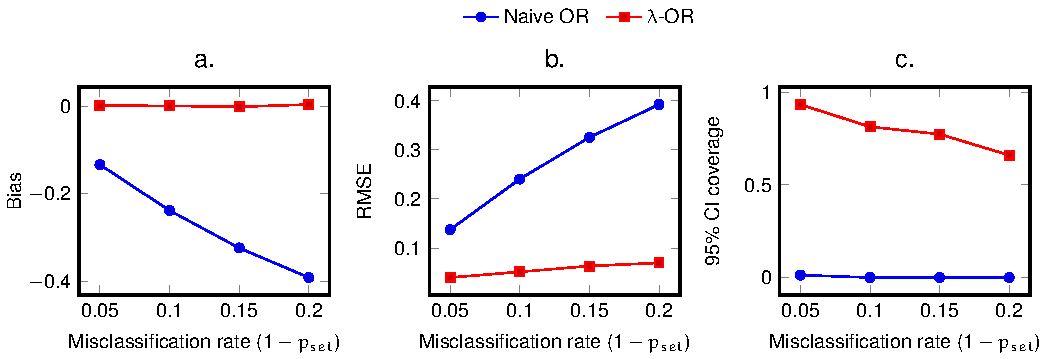
\includegraphics[width=\textwidth]{Figures/External/figsim}
  \fi

\caption{Finite-sample performance under two outcome-misclassification regimes.
Top row (panels a--d): specificity degradation with fixed \(p_{\mathrm{sel}}=0.95\) and varying false positive rate \(1-q_{\mathrm{sel}}\).
Bottom row (panels e--h): symmetric degradation with \(p_{\mathrm{sel}}=q_{\mathrm{sel}}\) and varying common misclassification rate \(m=1-p_{\mathrm{sel}}=1-q_{\mathrm{sel}}\).
Panels (a,e) show bias, (b,f) RMSE, and (c,g) nominal 95\% Wald coverage for naive log-OR and \(\log(\lambda\text{-OR})\).
Panels (d,h) show the conditioning diagnostic \(\det(K)=p_{\mathrm{sel}}+q_{\mathrm{sel}}-1\).}
\label{fig:spor_eight_panel}
\end{figure}
%################################### 
%###################################

\begin{figure}
\hspace{-15pt}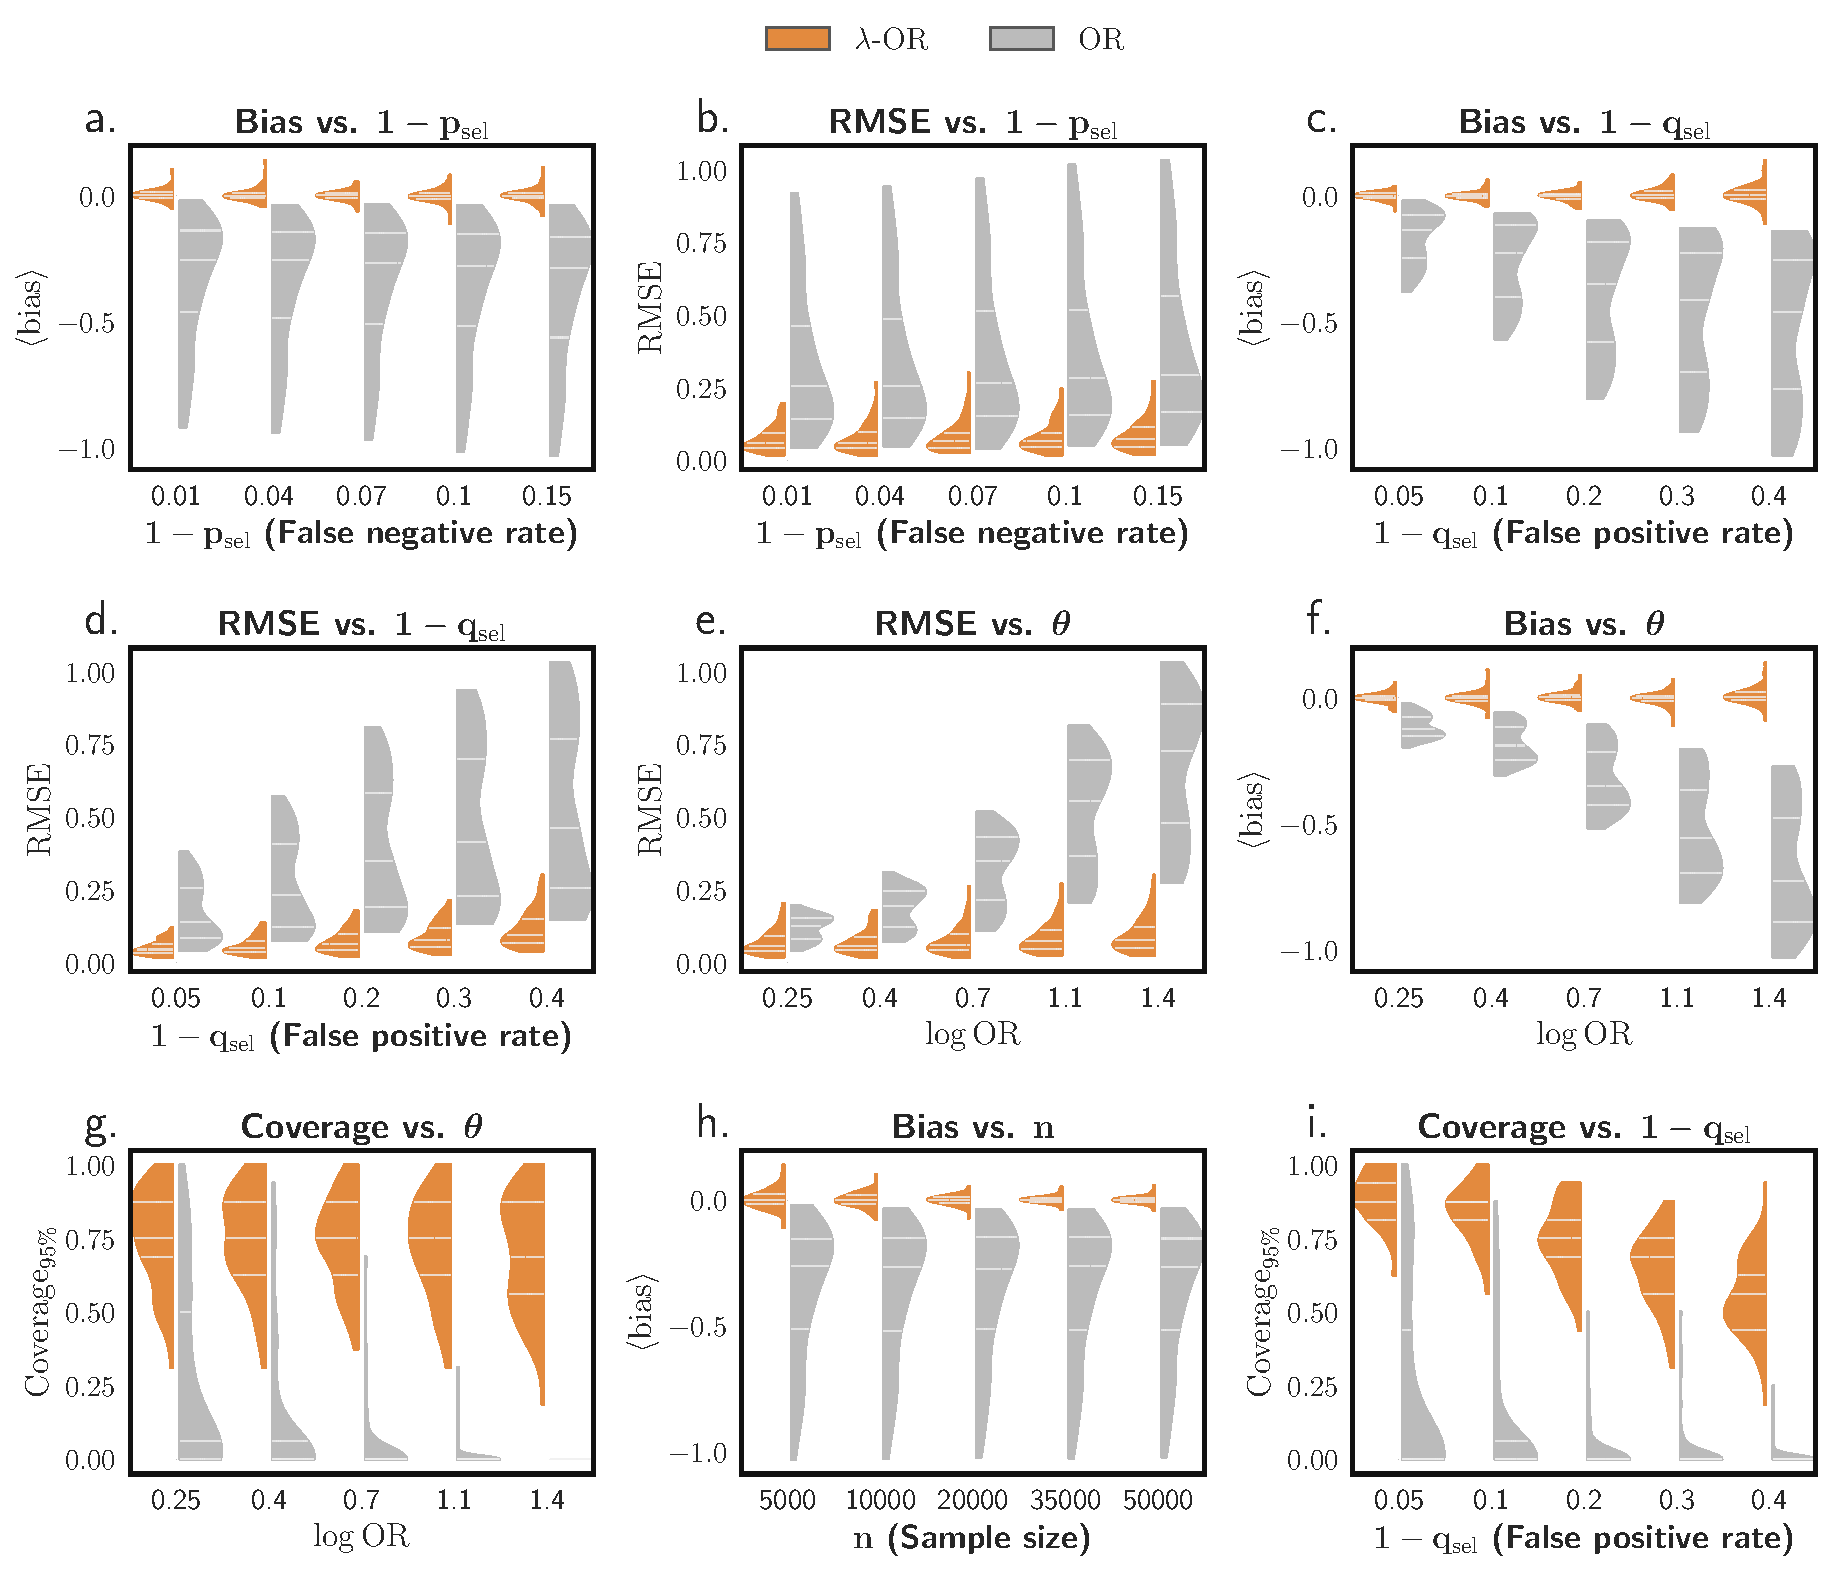
\includegraphics[width=1.05\textwidth]{../simulation/simulation_violin_grid.pdf}
\caption{\textbf{Simulation sweeps across misclassification, effect size, and sample size.}
Finite-sample performance of the naive log-odds ratio computed from the misclassified outcome table (OR; gray) and the corrected estimator \(\SPOR\) (red) obtained via ridge-stabilized inversion  (Algorithm~\ref{algo}). Each violin summarizes the distribution of bias, RMSE, or nominal 95\% Wald coverage (log scale) across \(R=250\) Monte Carlo replicates evaluated over randomly sampled combinations of simulation parameters drawn from predefined grids. Panels correspond to subsets of this grid emphasizing variation in the false negative rate \(1-p_{\mathrm{sel}}\) (a,b), the false positive rate \(1-q_{\mathrm{sel}}\) (c,d,i), the true log-odds effect \(\theta=\log(\mathrm{OR})\) (e,f,g), and the sample size \(n\) (h). Across sampled regimes the naive estimator exhibits systematic attenuation and rapid coverage collapse under outcome misclassification, whereas \(\SPOR\) remains substantially unbiased. Parameter grids and constants are listed in Tables~\ref{tab:sim_params} and~\ref{tab:sim_sweep_grids}.}\label{fig:sim_sweep_grid}\end{figure}

%###################################
%###################################

%%%%%\clearpage





\section{Simulation Study}\label{sec:sim}

\textbf{Purpose.}
We evaluate finite-sample behavior of the proposed misclassification-corrected odds ratio
(\(\SPOR\); Algorithm~\ref{algo}) against the naive log-odds ratio computed on the
misclassified outcome. The simulation isolates outcome misclassification and links
performance degradation to the conditioning of the misclassification operator,
summarized by \(\det(K)=p_{\mathrm{sel}}+q_{\mathrm{sel}}-1\) (Youden's \(J\)).
This connects directly to the collapse mechanism as \(J\to0\) formalized in
Theorems~\ref{thm:SPOR_collapse_J} and~\ref{thm:inherit_collapse}.

\textbf{Data-generating process (DGP) and target effect.}
Each replicate generates i.i.d.\ pairs \((X_i,Y_i)\) with \(X,Y\in\{0,1\}\).
We draw \(X\sim\mathrm{Bernoulli}(\varphi)\).
To enforce a prespecified target effect
\(\theta=\log(\mathrm{OR})\) and marginal outcome prevalence
\(\pi=\Pr(Y=1)\), we draw
\cgather{
Y\mid X \sim \mathrm{Bernoulli}\!\left(\mathrm{logit}^{-1}(\alpha+\theta X)\right),
}
with \(\alpha\) chosen numerically so that \(\Pr(Y=1)=\pi\).
From each replicate we form the latent \(2\times2\) contingency table
\(
T=\begin{bmatrix}
a & b\\
c & d
\end{bmatrix}
\)
using the indexing convention of Algorithm~\ref{algo}:
rows index \(X\in\{1,0\}\) and columns index the true outcome state
\(Y\in\{1,0\}\), i.e.,
\(a=\#\{X{=}1,Y{=}1\}\),
\(b=\#\{X{=}1,Y{=}0\}\),
\(c=\#\{X{=}0,Y{=}1\}\),
\(d=\#\{X{=}0,Y{=}0\}\).

\textbf{Outcome misclassification.}
Observed outcomes \(\tilde Y\) are generated from \(Y\) via independent,
non-differential flips with
\(p_{\mathrm{sel}}=\Pr(\tilde Y=1\mid Y=1)\)
and
\(q_{\mathrm{sel}}=\Pr(\tilde Y=0\mid Y=0)\),
using the same misclassification operator \(K\) as in the Methods
(Algorithm~\ref{algo}).
The observed table
\(
\tilde T=\begin{bmatrix}
\tilde a & \tilde b\\
\tilde c & \tilde d
\end{bmatrix}
\)
uses the same row/column convention.
Under Assumption~A, the mapping between \(T\) and \(\tilde T\) holds in expectation with a single operator \(K\),
whose conditioning is summarized by
\(\det(K)=p_{\mathrm{sel}}+q_{\mathrm{sel}}-1\).

\textbf{Estimators and uncertainty.}
The naive estimator is the classical log-odds ratio computed from
\(\tilde T\) with a \(0.5\) continuity correction.
The corrected estimator \(\SPOR\) is computed exactly as in
Algorithm~\ref{algo} by applying the stabilized right-inverse based on \(K\).
Equivalently, the corrected table is obtained from the ridge-stabilized inversion
described in Methods and Eq.~\eqref{eq:spor_corrected_table}.
The smallest \(\lambda\) on the feasibility grid yielding corrected cells above
the numerical floor \(\varepsilon\) is selected
(Table~\ref{tab:sim_params}); if none satisfies the constraint,
the largest \(\lambda\) is used and remaining sub-\(\varepsilon\)
cells are floored.
Nominal Wald standard errors for coverage are computed from the corrected cell counts.
The additional delta-method contribution arising when
\((p_{\mathrm{sel}},q_{\mathrm{sel}})\) are estimated from validation data is derived
separately in \ref{app:variance}; in the experiments below these
quantities are treated as fixed unless explicitly stated otherwise.

\textbf{Performance metrics.}
Across \(R\) replicates, for an estimator \(\widehat\ell\) of \(\theta\),
we compute bias, root mean squared error (RMSE), and nominal \(95\%\) Wald coverage on the log scale.
We also report the conditioning diagnostic
\(\det(K)=p_{\mathrm{sel}}+q_{\mathrm{sel}}-1\).
All constants, numerical safeguards, and base grids are specified in
Table~\ref{tab:sim_params}.

\textbf{Structured conditioning sweeps.}
Figure~\ref{fig:spor_eight_panel} presents two structured sweeps designed to
illustrate the theoretical conditioning mechanism.
In the specificity-degradation regime (top row),
we fix \(p_{\mathrm{sel}}=0.95\) and increase the false positive rate
\(1-q_{\mathrm{sel}}\).
As \(\det(K)\) decreases, the naive log-OR exhibits increasing attenuation,
RMSE inflation, and near-zero nominal coverage.
In contrast, \(\SPOR\) remains approximately unbiased and retains
substantially improved coverage over the well-conditioned regime,
with gradual variance-driven degradation as operator conditioning worsens.
In the symmetric-degradation regime (bottom row),
we impose \(p_{\mathrm{sel}}=q_{\mathrm{sel}}\) and sweep the common
misclassification rate
\(m=1-p_{\mathrm{sel}}=1-q_{\mathrm{sel}}\),
so that
\(\det(K)=1-2m\) decreases linearly.
This sweep makes the conditioning--performance relationship explicit,
and instability emerges as \(J\to0\),
consistent with the collapse mechanism proved in
Theorems~\ref{thm:SPOR_collapse_J} and~\ref{thm:inherit_collapse}.

\textbf{Expanded grid experiments.}
Figure~\ref{fig:sim_sweep_grid} extends the analysis by aggregating results
across a larger set of simulation runs generated by randomly sampling
parameter combinations
\((p_{\mathrm{sel}},q_{\mathrm{sel}},\theta,n)\)
from the grids listed in Table~\ref{tab:sim_sweep_grids}.
For each sampled configuration we generate \(R=250\) replicates and compute
the performance metrics above.
The violin plots therefore summarize variability across both Monte Carlo
replicates and sampled parameter configurations.
Panels group results according to the dominant varying quantity,
emphasizing the effects of the false negative rate \(1-p_{\mathrm{sel}}\),
the false positive rate \(1-q_{\mathrm{sel}}\),
the true log-odds effect \(\theta=\log(\mathrm{OR})\),
and the sample size \(n\).
Across these sampled regimes the naive estimator consistently exhibits
attenuation and rapid coverage collapse under outcome misclassification,
whereas \(\SPOR\) remains approximately unbiased over the well-conditioned
region and degrades gradually as \(\det(K)\to0\).

\begin{table}[t]
\centering
\caption{Fully specified simulation parameters and numerical safeguards used in Section~\ref{sec:sim}.}
\label{tab:sim_params}
\begin{tabular}{p{0.3\textwidth} p{0.5\textwidth}}
\hline
Quantity & Value / description \\
\hline
Replicates per grid point & \(R=250\) \\
Sample size per replicate & \(n=20{,}000\) \\
Outcome prevalence & \(\pi=\Pr(Y=1)=0.2\) \\
Exposure prevalence & \(\varphi=\Pr(X=1)=0.5\) \\
Target effect & \(\theta=\log(\mathrm{OR})=\log 2\) \\
DGP for \(X\) & \(X\sim\mathrm{Bernoulli}(\varphi)\) \\
DGP for \(Y\mid X\) &
\(Y\mid X\sim\mathrm{Bernoulli}(\mathrm{logit}^{-1}(\alpha+\theta X))\), \(\alpha\) chosen so \(\Pr(Y=1)=\pi\) \\
How \(\alpha\) is chosen &
Deterministic numeric solve (grid search / root-find) to match \(\Pr(Y=1)=\pi\) \\
Misclassification model &
Independent flips: \(\Pr(\tilde Y{=}1\mid Y{=}1)=p_{\mathrm{sel}}\), \(\Pr(\tilde Y{=}0\mid Y{=}0)=q_{\mathrm{sel}}\) \\
Non-differential assumption &
\((p_{\mathrm{sel}},q_{\mathrm{sel}})\) do not depend on \(X\) \\
Conditioning diagnostic &
\(\det(K)=p_{\mathrm{sel}}+q_{\mathrm{sel}}-1\) (plotted in panels d and h of Fig.~\ref{fig:spor_eight_panel}) \\
Top-row grid (specificity sweep) &
Fix \(p_{\mathrm{sel}}=0.95\); 15 points for \(1-q_{\mathrm{sel}}\in[0.02,0.65]\) \\
Bottom-row grid (symmetric sweep) &
Set \(p_{\mathrm{sel}}=q_{\mathrm{sel}}\); 15 points for \(m=1-p_{\mathrm{sel}}\in[0.02,0.35]\) \\
Naive continuity correction &
Add \(0.5\) to each observed cell \((\tilde a,\tilde b,\tilde c,\tilde d)\) \\
Feasibility floor &
\(\varepsilon=10^{-9}\) (corrected cells required \(\ge \varepsilon\)) \\
Ridge grid &
\(\lambda\in\{0,10^{-6},10^{-5},10^{-4},10^{-3}\}\) \\
Ridge selection rule &
Choose smallest \(\lambda\) on grid yielding all corrected cells \(\ge\varepsilon\);
if none, use \(\max\lambda\) and floor remaining sub-\(\varepsilon\) cells to \(\varepsilon\) \\
Validation size (variance propagation) &
\(n_{\mathrm{val}}=5{,}000\) (used only for the delta-method experiment in \ref{app:variance}) \\
RNG seed & 20251005 \\
\hline
\end{tabular}
\end{table}

\begin{table}[t]
\centering
\caption{Additional sweep grids used in Figure~\ref{fig:sim_sweep_grid}. All other constants and safeguards are as in Table~\ref{tab:sim_params}.}
\label{tab:sim_sweep_grids}
\begin{tabular}{p{0.35\textwidth} p{0.55\textwidth}}
\hline
Sweep dimension & Grid (held-fixed quantities) \\
\hline
False negative rate sweep & \(1-p_{\mathrm{sel}}\in\{0.01,0.04,0.07,0.10,0.15\}\) (with \(q_{\mathrm{sel}}\) fixed) \\
False positive rate sweep & \(1-q_{\mathrm{sel}}\in\{0.05,0.10,0.20,0.30,0.40\}\) with \(p_{\mathrm{sel}}=0.95\) fixed \\
Target effect sweep & \(\theta=\log(\mathrm{OR})\in\{0.25,0.40,0.70,1.10,1.40\}\) (with \(n\) and \((p_{\mathrm{sel}},q_{\mathrm{sel}})\) fixed) \\
Sample size sweep & \(n\in\{5000,10000,20000,35000,50000\}\) (with \(\theta\) and \((p_{\mathrm{sel}},q_{\mathrm{sel}})\) fixed) \\
\hline
\end{tabular}
\end{table}

\begin{figure}
  \includegraphics[width=\textwidth]{Figures/sim2.pdf}
  \caption{Simulation analogue of the attribution volcano plots. Panel a uses the classical log-odds ratio with its standard large-sample variance computed from the observed contingency table. Panel b uses the same estimated effect sizes but evaluates significance using the \(\lambda\)-OR variance that incorporates the additional delta-method contribution from estimation uncertainty in \((p_{\mathrm{sel}},q_{\mathrm{sel}})\) (See Methods). The added variance term induces a non-vanishing uncertainty floor, compressing the vertical scale and preventing the extreme significance inflation seen under naive inference at very large cohort size. Simulation parameters are listed in Table~\ref{tab:sim-volcano-params}.}
  \label{figsim2}
\end{figure}

\begin{figure}
  
\includegraphics[width=\textwidth]{Figures/performance_summary_alpha_0p05.png}
  \caption{Simulation results illustrating the dependence of total discoveries, true positives (TP), false positives (FP), and false discovery rate (FDR) on cohort size at significance level \(\alpha=0.05\). As cohort size increases, the naive estimator accumulates many false positives, whereas the \(\lambda\)-OR estimator yields substantially improved false discovery control because the validation-induced variance component prevents uncontrolled significance inflation.}
  \label{figsim3}
\end{figure}

\subsection{Simulation analogue of the attribution volcano plots}\label{sec:sim-volcano}

To illustrate the statistical implications of the variance expansion developed in
Methods, we performed an additional simulation designed to reproduce the
structure of the attribution volcano plots shown in Fig.~\ref{figsim2}. The
objective of this experiment is to isolate the variance mechanism implied by the
\(\lambda\)-OR formulation and compare it to classical odds-ratio inference under
very large sample sizes.

Recall that the corrected estimator is obtained from the ridge-stabilized corrected
table in Eq.~\eqref{eq:spor_corrected_table}, while inference for the log-scale
estimator uses the variance decomposition described in Methods. Specifically, the classical sampling variance
depends only on the corrected contingency-table counts, whereas the
misclassification-corrected analysis additionally includes the delta-method term
arising from estimation of the selection-conditional misclassification rates
\((p_{\mathrm{sel}},q_{\mathrm{sel}})\). In the volcano plots below, the horizontal
coordinate is the estimated log-effect and statistical significance is computed
from the Wald statistic \(Z=\widehat\ell/SE\), where \(SE\) is computed either
using only the classical large-sample variance (naive OR) or using the total
variance that includes the validation-induced uncertainty term (\(\lambda\)-OR inference).

\paragraph{Simulation design.}
We simulated \(m=20{,}000\) binary exposures representing candidate diagnostic
features. For each feature \(j\), a true log-odds ratio $\beta_j$
was drawn from a small-effect distribution
\cgather{
\beta_j \sim |\mathcal{N}(0.06,0.03^2)|.
}
Baseline exposure prevalence among controls was generated on the logit scale
\cgather{
\mathrm{logit}(p_{0j}) \sim \mathcal{N}(-3.5,1.0^2),
}
and case prevalence was defined by
\cgather{
p_{1j}=\mathrm{expit}\bigl(\mathrm{logit}(p_{0j})+\beta_j\bigr).
}
Counts were then sampled from a large cohort consisting of
\cgather{
n_{\mathrm{case}} = 5\times 10^{5},
\qquad
n_{\mathrm{ctrl}} = 5\times 10^{5},
}
yielding contingency tables \((a_j,b_j,c_j,d_j)\) for each feature.
For each table we computed the classical log-odds ratio
\cgather{
\widehat{\log(\mathrm{OR})}_j=\log\!\left(\frac{a_j d_j}{b_j c_j}\right),
}
and evaluated significance using the two variance specifications described above.

To determine the magnitude of the delta-method variance contribution, we fixed the
conditioning of the misclassification operator
\cgather{
\det(K)=p_{\mathrm{sel}}+q_{\mathrm{sel}}-1
}
and the validation cohort size \(n_{\mathrm{val}}\), which governs estimation
uncertainty in \((p_{\mathrm{sel}},q_{\mathrm{sel}})\). The parameters used in the
simulation are summarized in Table~\ref{tab:sim-volcano-params}.

The resulting volcano plots are shown in Fig.~\ref{figsim2}. Panel~a displays
the naive analysis using only the classical large-sample variance, whereas
panel~b shows significance computed using the total variance that includes the
additional validation-induced term.


Importantly, in these volcano plots, the vertical position of each exposure is determined by the  estimated variance of the $\lambda$-OR estimator. Consequently, the uncertainty of the corrected estimator directly governs which signals cross significance thresholds and are prioritized for follow-up investigation. Exposures with large positive $\lambda$-OR values and stable uncertainty correspond to candidate risk factors, whereas exposures with negative $\lambda$-OR values that remain significant after correction would  indicate candidate protective associations. %Thus the $\lambda$-OR variance provides a natural uncertainty-aware mechanism for prioritizing signals in large-scale screening analyses.

Under the classical estimator (Fig.~\ref{figsim2}a), the extremely large cohort
size causes the Wald variance to shrink toward zero, producing extremely large
test statistics even for modest effect sizes. As a result, a broad cloud of
features appears highly significant despite the small underlying effects.

In contrast, the \(\lambda\)-OR variance formulation incorporates the additional
delta-method term arising from estimation of \((p_{\mathrm{sel}},q_{\mathrm{sel}})\).
Because this component depends on the validation cohort rather than the primary
cohort, it imposes a lower bound on the achievable standard error. Consequently,
the volcano plot in Fig.~\ref{figsim2}b exhibits a substantially compressed
vertical scale in which statistical significance increases smoothly with effect
magnitude rather than diverging with sample size.

This experiment therefore provides a controlled demonstration that  the variance expansion
introduces a sample-size-independent component that prevents the collapse of
standard errors characteristic of classical odds-ratio inference in very large
observational datasets.

\paragraph{Cohort-size sweep.}
To examine how cohort size influences false discovery behavior under outcome
misclassification, we performed a sweep over case cohort sizes while holding all
other simulation parameters fixed. The number of cases was varied logarithmically
from \(10^{2}\) to \(10^{6}\) using 11 evenly spaced points on the log scale.
For each configuration, the control cohort size was set to
\(n_{\mathrm{ctrl}} = 100\, n_{\mathrm{case}}\). The total number of candidate
features was fixed at \(m=20{,}000\), of which a fraction \(0.8\) were null
features. Non-null effect sizes were sampled from
\(\mathcal{N}(0.06,\,0.03^{2})\).

Outcome misclassification parameters and validation sample size were held constant
across the sweep. Specifically, we used \(\epsilon = 0.8\),
\(n_{\mathrm{val}} = 1000\), and variance scaling factor \(1.0\), thereby inducing
the same validation-controlled uncertainty floor described above. Statistical
significance was evaluated at level \(\alpha = 0.05\).

For each cohort size, we computed discoveries using both the naive log-odds ratio
and the proposed misclassification-corrected estimator \(\log(\lambda\text{-OR})\).
We recorded the total number of discoveries, true positives (TP), false positives
(FP), and the resulting false discovery rate (FDR). Results are summarized in
Fig.~\ref{figsim3}.





The naive estimator exhibits a characteristic large-sample pathology. As
\(n_{\mathrm{case}}\) increases, the number of discoveries grows rapidly, driven
primarily by a large and persistent number of false positives. Consequently,
although statistical power increases with sample size, the associated FDR remains
elevated across much of the sweep.

In contrast, the \(\lambda\)-OR estimator shows markedly different scaling
behavior. Because the estimator incorporates the validation-induced variance floor, significance cannot
increase arbitrarily with cohort size. As \(n_{\mathrm{case}}\) increases, the
number of false positives declines sharply, approaching zero at the largest
cohort sizes examined. The resulting FDR correspondingly decreases and approaches
the nominal significance level.

While the naive estimator achieves higher apparent power due to aggressive
significance inflation, this gain is accompanied by a large false positive burden.
The \(\lambda\)-OR estimator yields fewer total discoveries but substantially
improves error control, producing a smaller and more reliable set of detected
signals. Importantly, true positives continue to increase with cohort size under
\(\lambda\)-OR, albeit at a slower rate than the naive estimator, reflecting the
stabilizing effect of the validation-based variance component.

These results illustrate the central motivation for the \(\lambda\)-OR correction.
In large observational cohorts with outcome misclassification, classical
odds-ratio inference can produce spurious significance driven purely by sample
size. By incorporating the variance contribution arising from estimation of
misclassification parameters, the \(\lambda\)-OR estimator prevents uncontrolled
significance inflation and yields substantially improved false discovery behavior
as cohort size increases.

\begin{table}[t]
\centering
\caption{Parameters used in the volcano simulation shown in Fig.~\ref{figsim2}.}
\label{tab:sim-volcano-params}
\begin{tabular}{lll}
\hline
Parameter & Description & Value \\
\hline
\(m\) & Number of simulated exposures & \(20{,}000\) \\
\(n_{\mathrm{case}}\) & Number of cases & \(5\times10^{5}\) \\
\(n_{\mathrm{ctrl}}\) & Number of controls & \(5\times10^{5}\) \\
\(\beta_j\) distribution & True log-OR effects & \(|\mathcal{N}(0.06,0.03^2)|\) \\
\(\mathrm{logit}(p_0)\) distribution & Baseline exposure prevalence & \(\mathcal{N}(-3.5,1.0^2)\) \\
\(\det(K)\) & Conditioning of misclassification operator & \(0.8\) \\
\(n_{\mathrm{val}}\) & Validation cohort size & \(1000\) \\
Random seed & Simulation RNG seed & \(3\) \\
\hline
\end{tabular}
\end{table}





















%\clearpage                      %

%% %###################################
%% %###################################
%% \section{Simulation Study}\label{sec:sim}

%% \textbf{Purpose.}
%% We evaluate finite-sample behavior of the proposed misclassification-corrected odds ratio
%% (\(\SPOR\); Algorithm~\ref{algo}) against the naive log-odds ratio computed on the
%% misclassified outcome. The simulation isolates outcome misclassification and links
%% performance degradation to the conditioning of the misclassification operator,
%% summarized by \(\det(K)=p_{\mathrm{sel}}+q_{\mathrm{sel}}-1\) (Youden's \(J\)).
%% This connects directly to the collapse mechanism as \(J\to0\) formalized in
%% Theorems~\ref{thm:SPOR_collapse_J} and~\ref{thm:inherit_collapse}.

%% \textbf{Data-generating process (DGP) and target effect.}
%% Each replicate generates i.i.d.\ pairs \((X_i,Y_i)\) with \(X,Y\in\{0,1\}\).
%% We draw \(X\sim\mathrm{Bernoulli}(\varphi)\).
%% To enforce a prespecified target effect
%% \(\theta=\log(\mathrm{OR})\) and marginal outcome prevalence
%% \(\pi=\Pr(Y=1)\), we draw
%% \cgather{
%% Y\mid X \sim \mathrm{Bernoulli}\!\left(\mathrm{logit}^{-1}(\alpha+\theta X)\right),
%% }
%% with \(\alpha\) chosen numerically so that \(\Pr(Y=1)=\pi\).
%% From each replicate we form the latent \(2\times2\) contingency table
%% \(
%% T=\begin{bmatrix}
%% a & b\\
%% c & d
%% \end{bmatrix}
%% \)
%% using the indexing convention of Algorithm~\ref{algo}:
%% rows index \(X\in\{1,0\}\) and columns index the true outcome state
%% \(Y\in\{1,0\}\), i.e.,
%% \(a=\#\{X{=}1,Y{=}1\}\),
%% \(b=\#\{X{=}1,Y{=}0\}\),
%% \(c=\#\{X{=}0,Y{=}1\}\),
%% \(d=\#\{X{=}0,Y{=}0\}\).

%% \textbf{Outcome misclassification.}
%% Observed outcomes \(\tilde Y\) are generated from \(Y\) via independent,
%% non-differential flips with
%% \(p_{\mathrm{sel}}=\Pr(\tilde Y=1\mid Y=1)\)
%% and
%% \(q_{\mathrm{sel}}=\Pr(\tilde Y=0\mid Y=0)\),
%% using the same misclassification operator \(K\) as in the Methods
%% (Algorithm~\ref{algo}).
%% The observed table
%% \(
%% \tilde T=\begin{bmatrix}
%% \tilde a & \tilde b\\
%% \tilde c & \tilde d
%% \end{bmatrix}
%% \)
%% uses the same row/column convention.
%% Under Assumption~A, the mapping between \(T\) and \(\tilde T\) holds in expectation with a single operator \(K\),
%% whose conditioning is summarized by
%% \(\det(K)=p_{\mathrm{sel}}+q_{\mathrm{sel}}-1\).

%% \textbf{Estimators and uncertainty.}
%% The naive estimator is the classical log-odds ratio computed from
%% \(\tilde T\) with a \(0.5\) continuity correction.
%% The corrected estimator \(\SPOR\) is computed exactly as in
%% Algorithm~\ref{algo} by applying the stabilized right-inverse based on \(K\).
%% The smallest \(\lambda\) on the feasibility grid yielding corrected cells above
%% the numerical floor \(\varepsilon\) is selected
%% (Table~\ref{tab:sim_params}); if none satisfies the constraint,
%% the largest \(\lambda\) is used and remaining sub-\(\varepsilon\)
%% cells are floored.
%% Nominal Wald standard errors for coverage are computed from the corrected cell counts.
%% The additional delta-method contribution arising when
%% \((p_{\mathrm{sel}},q_{\mathrm{sel}})\) are estimated from validation data is derived
%% separately in Appendix~\ref{app:variance}; in the experiments below these
%% quantities are treated as fixed.

%% \textbf{Performance metrics.}
%% Across \(R\) replicates, for an estimator \(\widehat\ell\) of \(\theta\),
%% we compute bias, Root Mean Square Error (RMSE), and nominal \(95\%\) Wald coverage on the log scale.
%% We also report the conditioning diagnostic
%% \(\det(K)=p_{\mathrm{sel}}+q_{\mathrm{sel}}-1\).
%% All constants, numerical safeguards, and base grids are specified in
%% Table~\ref{tab:sim_params}.

%% \textbf{Structured conditioning sweeps.}
%% Figure~\ref{fig:spor_eight_panel} presents two structured sweeps designed to
%% illustrate the theoretical conditioning mechanism.
%% In the specificity-degradation regime (top row),
%% we fix \(p_{\mathrm{sel}}=0.95\) and increase the false positive rate
%% \(1-q_{\mathrm{sel}}\).
%% As \(\det(K)\) decreases, the naive log-OR exhibits increasing attenuation,
%% RMSE inflation, and near-zero nominal coverage.
%% In contrast, \(\SPOR\) remains approximately unbiased and retains
%% substantially improved coverage over the well-conditioned regime,
%% with gradual variance-driven degradation as operator conditioning worsens.
%% In the symmetric-degradation regime (bottom row),
%% we impose \(p_{\mathrm{sel}}=q_{\mathrm{sel}}\) and sweep the common
%% misclassification rate
%% \(m=1-p_{\mathrm{sel}}=1-q_{\mathrm{sel}}\),
%% so that
%% \(\det(K)=1-2m\) decreases linearly.
%% This sweep makes the conditioning–performance relationship explicit,
%% and instability emerges as \(J\to0\),
%% consistent with the collapse mechanism proved in
%% Theorems~\ref{thm:SPOR_collapse_J} and~\ref{thm:inherit_collapse}.

%% \textbf{Expanded grid experiments.}
%% Figure~\ref{fig:sim_sweep_grid} extends the analysis by aggregating results
%% across a larger set of simulation runs generated by randomly sampling
%% parameter combinations
%% \((p_{\mathrm{sel}},q_{\mathrm{sel}},\theta,n)\)
%% from the grids listed in Table~\ref{tab:sim_sweep_grids}.
%% For each sampled configuration we generate \(R=250\) replicates and compute
%% the performance metrics above.
%% The violin plots therefore summarize variability across both Monte Carlo
%% replicates and sampled parameter configurations.
%% Panels group results according to the dominant varying quantity,
%% emphasizing the effects of the false negative rate \(1-p_{\mathrm{sel}}\),
%% the false positive rate \(1-q_{\mathrm{sel}}\),
%% the true log-odds effect \(\theta=\log(\mathrm{OR})\),
%% and the sample size \(n\).
%% Across these sampled regimes the naive estimator consistently exhibits
%% attenuation and rapid coverage collapse under outcome misclassification,
%% whereas \(\SPOR\) remains approximately unbiased over the well-conditioned
%% region and degrades gradually as \(\det(K)\to0\).
%% %###################################
%% %###################################








%% %################################### 

%% \begin{table}[t]
%% \centering
%% \caption{Fully specified simulation parameters and numerical safeguards used in Section~\ref{sec:sim}.}
%% \label{tab:sim_params}
%% \begin{tabular}{p{0.3\textwidth} p{0.5\textwidth}}
%% \hline
%% Quantity & Value / description \\
%% \hline
%% Replicates per grid point & \(R=250\) \\
%% Sample size per replicate & \(n=20{,}000\) \\
%% Outcome prevalence & \(\pi=\Pr(Y=1)=0.2\) \\
%% Exposure prevalence & \(\varphi=\Pr(X=1)=0.5\) \\
%% Target effect & \(\theta=\log(\mathrm{OR})=\log 2\) \\
%% DGP for \(X\) & \(X\sim\mathrm{Bernoulli}(\varphi)\) \\
%% DGP for \(Y\mid X\) &
%% \(Y\mid X\sim\mathrm{Bernoulli}(\mathrm{logit}^{-1}(\alpha+\theta X))\), \(\alpha\) chosen so \(\Pr(Y=1)=\pi\) \\
%% How \(\alpha\) is chosen &
%% Deterministic numeric solve (grid search / root-find) to match \(\Pr(Y=1)=\pi\) \\
%% Misclassification model &
%% Independent flips: \(\Pr(\tilde Y{=}1\mid Y{=}1)=p_{\mathrm{sel}}\), \(\Pr(\tilde Y{=}0\mid Y{=}0)=q_{\mathrm{sel}}\) \\
%% Non-differential assumption &
%% \((p_{\mathrm{sel}},q_{\mathrm{sel}})\) do not depend on \(X\) \\
%% Conditioning diagnostic &
%% \(\det(K)=p_{\mathrm{sel}}+q_{\mathrm{sel}}-1\) (plotted in panels d and h of Fig.~\ref{fig:spor_eight_panel}) \\
%% Top-row grid (specificity sweep) &
%% Fix \(p_{\mathrm{sel}}=0.95\); 15 points for \(1-q_{\mathrm{sel}}\in[0.02,0.65]\) \\
%% Bottom-row grid (symmetric sweep) &
%% Set \(p_{\mathrm{sel}}=q_{\mathrm{sel}}\); 15 points for \(m=1-p_{\mathrm{sel}}\in[0.02,0.35]\) \\
%% Naive continuity correction &
%% Add \(0.5\) to each observed cell \((\tilde a,\tilde b,\tilde c,\tilde d)\) \\
%% Feasibility floor &
%% \(\varepsilon=10^{-9}\) (corrected cells required \(\ge \varepsilon\)) \\
%% Ridge grid &
%% \(\lambda\in\{0,10^{-6},10^{-5},10^{-4},10^{-3}\}\) \\
%% Ridge selection rule &
%% Choose smallest \(\lambda\) on grid yielding all corrected cells \(\ge\varepsilon\);
%% if none, use \(\max\lambda\) and floor remaining sub-\(\varepsilon\) cells to \(\varepsilon\) \\
%% Validation size (variance propagation) &
%% \(n_{\mathrm{val}}=5{,}000\) (used only for the delta-method experiment in Appendix~\ref{app:variance}) \\
%% RNG seed & 20251005 \\
%% \hline
%% \end{tabular}
%% \end{table}
%% %################################### 
%% \begin{table}[t]
%% \centering
%% \caption{Additional sweep grids used in Figure~\ref{fig:sim_sweep_grid}. All other constants and safeguards are as in Table~\ref{tab:sim_params}.}
%% \label{tab:sim_sweep_grids}
%% \begin{tabular}{p{0.35\textwidth} p{0.55\textwidth}}
%% \hline
%% Sweep dimension & Grid (held-fixed quantities) \\
%% \hline
%% False negative rate sweep & \(1-p_{\mathrm{sel}}\in\{0.01,0.04,0.07,0.10,0.15\}\) (with \(q_{\mathrm{sel}}\) fixed) \\
%% False positive rate sweep & \(1-q_{\mathrm{sel}}\in\{0.05,0.10,0.20,0.30,0.40\}\) with \(p_{\mathrm{sel}}=0.95\) fixed \\
%% Target effect sweep & \(\theta=\log(\mathrm{OR})\in\{0.25,0.40,0.70,1.10,1.40\}\) (with \(n\) and \((p_{\mathrm{sel}},q_{\mathrm{sel}})\) fixed) \\
%% Sample size sweep & \(n\in\{5000,10000,20000,35000,50000\}\) (with \(\theta\) and \((p_{\mathrm{sel}},q_{\mathrm{sel}})\) fixed) \\
%% \hline
%% \end{tabular}
%% \end{table}
%% %################################### 
%% %################################### 
%% %################################### 
%% %################################### 
%% %################################### 
%% %################################### 
%% %==================================================
%% %second sim study in Rev request
%% %==================================================

%% \begin{figure}

%%   \includegraphics[width=\textwidth]{Figures/sim2.pdf}

%%   \caption{}\label{figsim2}

%% \end{figure}



%% \begin{figure}

%%   
\includegraphics[width=\textwidth]{Figures/performance_summary_alpha_0p05.png}

%% \caption{Simulation results illustrating variation of FDR, true positives and false psitives with sample size}\label{figsim3}

%% \end{figure}

%====================================================
%====================================================
%%!!!!!!!!!!!!!!!!!!!!!!!!!!!!!!!!!!!!!!!!!!!!!!!!!!
%%!!!!!!!!!!!!!!!!!!!!!!!!!!!!!!!!!!!!!!!!!!!!!!!!!!
%%!!!!!!!!!!!!!!!!!!!!!!!!!!!!!!!!!!!!!!!!!!!!!!!!!!
%%!!!!!!!!!!!!!!!!!!!!!!!!!!!!!!!!!!!!!!!!!!!!!!!!!!
%====================================================
%====================================================



%==================================================
% Additional simulation requested in revision
%==================================================

%% \begin{figure}[t]
%%   \centering
%%   \includegraphics[width=\textwidth]{Figures/sim2.pdf}
%%   \caption{
%%   Simulation analogue of attribution volcano plots under naive and $\lambda$-OR inference.
%%   Each point represents one simulated binary feature; red points denote non-null features
%%   and green points denote null features. The horizontal axis is the estimated log-effect,
%%   and the vertical axis is statistical significance measured by $-\log_{10}(p)$ from a Wald
%%   test. Panels (a,c,e) show naive log-odds-ratio inference using only the classical
%%   sampling variance, while panels (b,d,f) show $\lambda$-OR inference using the augmented
%%   variance that includes the validation-driven uncertainty contribution. Results are shown
%%   for three cohort sizes: $n_{\mathrm{case}}=n_{\mathrm{ctrl}}=5\times 10^{4}$ in panels
%%   (a,b), $10^{5}$ in panels (c,d), and $10^{6}$ in panels (e,f). As sample size increases,
%%   the naive analysis produces increasingly inflated significance even for weak effects,
%%   whereas $\lambda$-OR compresses the vertical scale through the additional variance term
%%   and preserves a more stable separation between null and non-null features.
%%   }
%%   \label{figsim2}
%% \end{figure}

%% \begin{figure}[t]
%%   \centering
%%   
\includegraphics[width=\textwidth]{Figures/performance_summary_alpha_0p05.png}
%%   \caption{
%%   Cohort-size sweep at significance level $\alpha=0.05$. The number of cases
%%   $n_{\mathrm{case}}$ is varied logarithmically from $10^{2}$ to $10^{6}$ using 11
%%   evenly spaced points on the log scale, with $n_{\mathrm{ctrl}}=100\,n_{\mathrm{case}}$
%%   throughout. Panels show the false discovery rate (FDR), the number of true positives
%%   (TP), and the number of false positives (FP) for naive odds-ratio inference and
%%   $\lambda$-OR inference. As cohort size increases, naive inference accumulates a large
%%   and persistent false-positive burden, whereas $\lambda$-OR sharply reduces false
%%   positives and correspondingly lowers FDR while still increasing the number of true
%%   positives.}
%%   \label{figsim3}
%% \end{figure}

%% \subsection{Simulation analogue of the attribution volcano plots}\label{sec:sim-volcano}

%% To complement the finite-sample misclassification experiments above, we performed an
%% additional simulation designed to reproduce the geometry of the attribution volcano
%% plots used in the empirical analyses. The purpose of this experiment is not to study
%% bias of the corrected point estimator itself, but to isolate the inferential consequence
%% of the variance expansion developed in Section~2.3. In particular, the experiment
%% illustrates how the additional uncertainty induced by estimation of
%% $(p_{\mathrm{sel}},q_{\mathrm{sel}})$ prevents the collapse of standard errors that occurs
%% under classical odds-ratio inference in very large cohorts.

%% We simulated $m=20{,}000$ binary exposures representing candidate diagnostic features.
%% A fraction $0.8$ of these were designated null features, with true effect
%% $\beta_j=0$, and the remaining features were assigned non-null effects drawn from
%% \[
%% \beta_j \sim \mathcal{N}(0.06,\,0.03^2).
%% \]
%% Baseline exposure prevalence among controls was generated on the logit scale as
%% \[
%% \operatorname{logit}(p_{0j}) \sim \mathcal{N}(-3.5,\,1.0^2),
%% \]
%% and case prevalence was then defined by
%% \[
%% p_{1j}=\operatorname{expit}\!\bigl(\operatorname{logit}(p_{0j})+\beta_j\bigr).
%% \]
%% For each feature $j$, counts $(a_j,b_j,c_j,d_j)$ were sampled from independent
%% case and control cohorts, and the naive log-odds ratio
%% \[
%% \widehat{\ell}^{\,\mathrm{naive}}_j
%% =
%% \log\!\left(\frac{a_j d_j}{b_j c_j}\right)
%% \]
%% was computed in the usual way.

%% We then evaluated statistical significance under two variance models. In the naive
%% analysis, the Wald statistic uses only the classical large-sample variance of the
%% log-odds ratio. In the $\lambda$-OR analysis, inference uses the total variance obtained
%% by augmenting the classical term with the additional contribution arising from
%% uncertainty in the selection-conditional misclassification rates
%% $(p_{\mathrm{sel}},q_{\mathrm{sel}})$. In the simulation, this extra term was parameterized
%% through the conditioning quantity
%% \[
%% \det(K)=p_{\mathrm{sel}}+q_{\mathrm{sel}}-1
%% \]
%% and a finite validation cohort of size $n_{\mathrm{val}}$, yielding a validation-driven
%% standard-error floor that does not vanish with the primary cohort size.

%% Figure~\ref{figsim2} shows the resulting volcano plots for three cohort sizes:
%% $n_{\mathrm{case}}=n_{\mathrm{ctrl}}=5\times10^{4}$,
%% $n_{\mathrm{case}}=n_{\mathrm{ctrl}}=10^{5}$, and
%% $n_{\mathrm{case}}=n_{\mathrm{ctrl}}=10^{6}$.
%% Under naive inference, the increasing cohort size drives the Wald variance toward
%% zero, so even modest effect sizes produce increasingly large test statistics and a broad
%% cloud of apparently significant findings. This inflation affects null and non-null
%% features alike, obscuring the distinction between weak signal and spurious discovery.
%% In contrast, under $\lambda$-OR inference the validation-induced variance component
%% imposes a lower bound on the achievable standard error. The resulting volcano plots
%% therefore exhibit a markedly compressed vertical scale in which significance grows much
%% more slowly with cohort size and remains more tightly coupled to effect magnitude.

%% This experiment isolates the core inferential mechanism of the method. The benefit
%% does not come from altering the basic odds-ratio geometry of the feature tables, but
%% from propagating uncertainty in the misclassification correction into the final test
%% statistic. In very large observational datasets, this additional variance component
%% prevents the pathological over-certainty that otherwise turns weak or null associations
%% into apparently overwhelming discoveries.

%% \paragraph{Cohort-size sweep at fixed significance threshold.}
%% To quantify the large-sample behavior more directly, we next performed a cohort-size
%% sweep while holding all other simulation parameters fixed and evaluating discoveries at
%% significance level $\alpha=0.05$. The number of cases was varied logarithmically from
%% $10^{2}$ to $10^{6}$ using 11 evenly spaced points on the log scale, with
%% $n_{\mathrm{ctrl}} = 100\,n_{\mathrm{case}}$ for each configuration. The total number of
%% candidate features remained fixed at $m=20{,}000$, with null fraction $0.8$, non-null
%% effect distribution $\mathcal{N}(0.06,0.03^2)$, conditioning level $\det(K)=0.8$,
%% validation sample size $n_{\mathrm{val}}=1000$, and variance scaling factor $1.0$.

%% For each cohort size we recorded the number of discoveries, true positives (TP), false
%% positives (FP), and the resulting false discovery rate
%% \[
%% \mathrm{FDR}=\frac{\mathrm{FP}}{\mathrm{TP}+\mathrm{FP}}
%% \]
%% under both naive odds-ratio inference and $\lambda$-OR inference. The results are
%% summarized in Fig.~\ref{figsim3}.

%% The naive analysis exhibits the characteristic large-sample failure mode anticipated by
%% the variance calculation. As $n_{\mathrm{case}}$ increases, the number of true positives
%% does rise, but this is accompanied by a persistently large false-positive burden.
%% Consequently, the false discovery rate remains high over much of the sweep, indicating
%% that the apparent gain in power is achieved largely through significance inflation.
%% By contrast, $\lambda$-OR inference shows a different scaling regime. Because the
%% validation-driven variance component does not shrink with the main cohort size, false
%% positives decline sharply as $n_{\mathrm{case}}$ increases, and the false discovery rate
%% falls correspondingly. At the same time, the number of true positives continues to
%% increase, although more gradually than under the naive analysis.

%% Taken together, Figs.~\ref{figsim2} and~\ref{figsim3} show that the additional
%% variance term is not merely a technical correction. It changes the qualitative
%% large-sample behavior of the inference procedure. Classical odds-ratio inference on
%% misclassification-corrected tables can still produce severe over-significance when the
%% primary cohort is extremely large, whereas $\lambda$-OR inference stabilizes the test
%% statistic by retaining the uncertainty associated with estimation of the correction
%% itself.

%% \begin{table}[!ht]
%% \centering
%% \caption{Parameters used in the additional volcano-style simulation and the associated
%% cohort-size sweep in Section~\ref{sec:sim-volcano}. Unless otherwise noted, the same
%% values are used for both experiments.}
%% \label{tab:sim-volcano-params}
%% \begin{tabular}{p{0.34\textwidth} p{0.56\textwidth}}
%% \hline
%% Parameter / quantity & Value / description \\
%% \hline
%% Number of simulated exposures & $m=20{,}000$ \\
%% Null fraction & $0.8$ \\
%% Non-null effect distribution & $\beta_j \sim \mathcal{N}(0.06,\,0.03^2)$ \\
%% Null effect & $\beta_j = 0$ \\
%% Baseline exposure prevalence & $\operatorname{logit}(p_{0j}) \sim \mathcal{N}(-3.5,\,1.0^2)$ \\
%% Case prevalence for feature $j$ & $p_{1j}=\operatorname{expit}(\operatorname{logit}(p_{0j})+\beta_j)$ \\
%% Conditioning of misclassification operator & $\det(K)=0.8$ \\
%% Validation cohort size & $n_{\mathrm{val}}=1000$ \\
%% Variance scaling factor & $1.0$ \\
%% Random seed & $3$ \\
%% Volcano-plot cohort sizes & $n_{\mathrm{case}}=n_{\mathrm{ctrl}} \in \{5\times10^{4},\,10^{5},\,10^{6}\}$ \\
%% Cohort-size sweep & $n_{\mathrm{case}} \in [10^{2},10^{6}]$ on a log scale with 11 points \\
%% Control size in sweep & $n_{\mathrm{ctrl}} = 100\,n_{\mathrm{case}}$ \\
%% Significance threshold for sweep & $\alpha = 0.05$ \\
%% Reported sweep metrics & discoveries, TP, FP, FDR \\
%% \hline
%% \end{tabular}
%% \end{table}













%====================================================
%====================================================
%%!!!!!!!!!!!!!!!!!!!!!!!!!!!!!!!!!!!!!!!!!!!!!!!!!!
%%!!!!!!!!!!!!!!!!!!!!!!!!!!!!!!!!!!!!!!!!!!!!!!!!!!
%%!!!!!!!!!!!!!!!!!!!!!!!!!!!!!!!!!!!!!!!!!!!!!!!!!!
%%!!!!!!!!!!!!!!!!!!!!!!!!!!!!!!!!!!!!!!!!!!!!!!!!!!
%%!!!!!!!!!!!!!!!!!!!!!!!!!!!!!!!!!!!!!!!!!!!!!!!!!!
%%!!!!!!!!!!!!!!!!!!!!!!!!!!!!!!!!!!!!!!!!!!!!!!!!!!
%%!!!!!!!!!!!!!!!!!!!!!!!!!!!!!!!!!!!!!!!!!!!!!!!!!!
%%!!!!!!!!!!!!!!!!!!!!!!!!!!!!!!!!!!!!!!!!!!!!!!!!!!
%%!!!!!!!!!!!!!!!!!!!!!!!!!!!!!!!!!!!!!!!!!!!!!!!!!!
%%!!!!!!!!!!!!!!!!!!!!!!!!!!!!!!!!!!!!!!!!!!!!!!!!!!
%%!!!!!!!!!!!!!!!!!!!!!!!!!!!!!!!!!!!!!!!!!!!!!!!!!!
%%!!!!!!!!!!!!!!!!!!!!!!!!!!!!!!!!!!!!!!!!!!!!!!!!!!
%====================================================
%====================================================
%====================================================
%====================================================

%% \subsection{Simulation analogue of the attribution volcano plots}\label{sec:sim-volcano}
%% To illustrate the statistical implications of the variance expansion developed in
%% Section~2.3, we performed an additional simulation designed to reproduce the
%% structure of the attribution volcano plots shown in Fig.~\ref{figsim2}.  The
%% objective of this experiment is to isolate the variance mechanism implied by the
%% $\lambda$-OR formulation and compare it to classical odds-ratio inference under
%% very large sample sizes.

%% Recall that the $\lambda$-OR estimator is obtained from the corrected contingency
%% table in Eq.~(7), while inference for the log-scale estimator uses the variance
%% expression derived in Section~2.3.  Specifically, the classical sampling variance
%% of the log-odds ratio is given by Eq.~(8), while the additional uncertainty arising
%% from estimation of the selection--conditional misclassification rates
%% $(p_{\mathrm{sel}},q_{\mathrm{sel}})$ is captured by the delta-method term in
%% Eq.~(9).  The total variance used for inference is therefore the sum in Eq.~(10).
%% In the volcano plots below, the horizontal coordinate is the estimated
%% log-effect $\log(\mathrm{OR})$ and statistical significance is computed from the
%% Wald statistic $Z=\frac{\log(\mathrm{OR})}{SE}$, where $SE$ is computed either using only the classical variance in Eq.~(8)
%% (naive OR) or the total variance in Eq.~(10) ($\lambda$-OR inference).

%% \paragraph{Simulation design.}
%% We simulated $m=20{,}000$ binary exposures representing candidate diagnostic
%% features.  For each feature $j$, a true log-odds ratio
%% \[
%% \beta_j
%% \]
%% was drawn from a small-effect distribution
%% \[
%% \beta_j \sim |\mathcal{N}(0.06,0.03^2)|.
%% \]
%% Baseline exposure prevalence among controls was generated on the logit scale
%% \[
%% \mathrm{logit}(p_{0j}) \sim \mathcal{N}(-3.5,1.0^2),
%% \]
%% and case prevalence was defined by
%% \[
%% p_{1j}=\mathrm{expit}\bigl(\mathrm{logit}(p_{0j})+\beta_j\bigr).
%% \]

%% Counts were then sampled from a large cohort consisting of
%% \[
%% n_{\mathrm{case}} = 5\times 10^{5},
%% \qquad
%% n_{\mathrm{ctrl}} = 5\times 10^{5},
%% \]
%% yielding contingency tables $(a_j,b_j,c_j,d_j)$ for each feature.
%% For each table we computed the classical log-odds ratio
%% \[
%% \widehat{\log(\mathrm{OR})}_j=\log\!\left(\frac{a_j d_j}{b_j c_j}\right)
%% \]
%% and evaluated significance using the two variance estimators described above.

%% To determine the magnitude of the delta-method variance term in
%% Eq.~(9), we fixed the conditioning of the misclassification operator
%% \[
%% \det(K)=p_{\mathrm{sel}}+q_{\mathrm{sel}}-1
%% \]
%% and the validation cohort size $n_{\mathrm{val}}$ that governs estimation
%% uncertainty in $(p_{\mathrm{sel}},q_{\mathrm{sel}})$.  The parameters used in the
%% simulation are summarized in Table~\ref{tab:sim-volcano-params}.


%% %\paragraph{Results.}
%% The resulting volcano plots are shown in Fig.~\ref{figsim2}.  Panel
%% \ref{figsim2}a displays the naive analysis using the classical variance
%% (Eq.~(8)), while panel \ref{figsim2}b shows significance computed using the
%% total variance from Eq.~(10).

%% Under the classical estimator (Fig.~\ref{figsim2}a), the extremely large cohort
%% size causes the Wald variance to shrink toward zero, producing extremely large
%% test statistics even for modest effect sizes.  As a result, a broad cloud of
%% features appears highly significant despite the small underlying effects.

%% In contrast, the $\lambda$-OR variance formulation incorporates the additional
%% delta-method term arising from estimation of $(p_{\mathrm{sel}},q_{\mathrm{sel}})$.
%% Because this component depends on the validation cohort rather than the primary
%% cohort, it imposes a lower bound on the achievable standard error.  Consequently,
%% the volcano plot in Fig.~\ref{figsim2}b exhibits a substantially compressed
%% vertical scale in which statistical significance increases smoothly with effect
%% magnitude rather than diverging with sample size.

%% This experiment therefore provides a controlled demonstration of the mechanism
%% highlighted in Section~2.3: the variance expansion in Eq.~(10) introduces a
%% sample-size–independent variance component that prevents the collapse of
%% standard errors characteristic of classical odds-ratio inference in very large
%% observational datasets.


%% \paragraph{Cohort-size sweep.}
%% To examine how cohort size influences false discovery behavior under outcome misclassification, we performed a sweep over case cohort sizes while holding all other simulation parameters fixed. The number of cases was varied logarithmically from $10^{2}$ to $10^{6}$ using 11 evenly spaced points on the log scale. For each configuration, the control cohort size was set to $n_{\mathrm{ctrl}} = 100\, n_{\mathrm{case}}$. The total number of candidate features was fixed at $m=20{,}000$, of which a fraction $0.8$ were null features. Non-null effect sizes were sampled from $\mathcal{N}(0.06,\,0.03^{2})$. %Baseline prevalences were drawn from the distribution described in Section~\ref{sec:sim}.

%% Outcome misclassification parameters and validation sample size were held constant across the sweep. Specifically, we used $\epsilon = 0.8$, $n_{\mathrm{val}} = 1000$, and variance scaling factor $1.0$, resulting in a validation-induced variance floor of the form described in Eq.~(\ref{eq:lambda_var}). Statistical significance was evaluated at level $\alpha = 0.05$.

%% For each cohort size, we computed discoveries using both the naive log-odds ratio and the proposed misclassification-corrected estimator $\log(\lambda\text{-OR})$. We recorded the total number of discoveries, true positives (TP), false positives (FP), and the resulting false discovery rate (FDR). Results are summarized in Fig.~\ref{figsim3}.

%% %% \paragraph{Observed behavior.}  %
%% The naive estimator exhibits a characteristic large-sample pathology. As $n_{\mathrm{case}}$ increases, the number of discoveries grows rapidly, driven primarily by a large and persistent number of false positives. Consequently, although statistical power increases with sample size, the associated FDR remains elevated across much of the sweep.

%% In contrast, the $\lambda$-OR estimator shows markedly different scaling behavior. Because the estimator incorporates the validation-induced variance floor described in Section~\ref{sec:methods}, significance cannot increase arbitrarily with cohort size. As $n_{\mathrm{case}}$ increases, the number of false positives declines sharply, approaching zero at the largest cohort sizes examined. The resulting FDR correspondingly decreases and approaches the nominal significance level.

%% %% \paragraph{Power and error tradeoff.}
%% While the naive estimator achieves higher apparent power due to aggressive significance inflation, this gain is accompanied by a large false positive burden. The $\lambda$-OR estimator yields fewer total discoveries but substantially improves error control, producing a smaller and more reliable set of detected signals. Importantly, true positives continue to increase with cohort size under $\lambda$-OR, albeit at a slower rate than the naive estimator, reflecting the stabilizing effect of the validation-based variance component.

%% %% \paragraph{Interpretation.}
%% These results illustrate the central motivation for the $\lambda$-OR correction. In large observational cohorts with outcome misclassification, classical odds-ratio inference can produce spurious significance driven purely by sample size. By incorporating the variance contribution arising from estimation of misclassification parameters, the $\lambda$-OR estimator prevents uncontrolled significance inflation and yields substantially improved false discovery behavior as cohort size increases.


%% \begin{table}[t]
%% \centering
%% \caption{Parameters used in the volcano simulation shown in
%% Fig.~\ref{figsim2}.}
%% \label{tab:sim-volcano-params}
%% \begin{tabular}{lll}
%% \hline
%% Parameter & Description & Value \\
%% \hline
%% $m$ & Number of simulated exposures & $20{,}000$ \\
%% $n_{\mathrm{case}}$ & Number of cases & $5\times10^{5}$ \\
%% $n_{\mathrm{ctrl}}$ & Number of controls & $5\times10^{5}$ \\
%% $\beta_j$ distribution & True log-OR effects & $|\mathcal{N}(0.06,0.03^2)|$ \\
%% $\mathrm{logit}(p_0)$ distribution & Baseline exposure prevalence & $\mathcal{N}(-3.5,1.0^2)$ \\
%% $\det(K)$ & Conditioning of misclassification operator & $0.8$ \\
%% $n_{\mathrm{val}}$ & Validation cohort size & $1000$ \\
%% Random seed & Simulation RNG seed & $3$ \\
%% \hline
%% \end{tabular}
%% \end{table}











%################################### 
%################################### 
\begin{figure}[!ht]
\centering 
  \tikzexternalenable
  \tikzsetnextfilename{figvolcano}

%\tikzXtrue
  \iftikzX
  \begin{tikzpicture}[font=\bf\sffamily\fontsize{10}{10}\selectfont]
    \def\WDT{\textwidth}
    \node[] (A) at (0,0) {
\includegraphics[width=\WDT]{Figures/figcompsemilogIPF}};
    \node[anchor=north west] (B) at ([yshift=.1in]A.south west) {
\includegraphics[width=\WDT]{Figures/figcompsemilogASD}};
    \node[anchor=north west] (C) at ([yshift=.1in]B.south west) {
\includegraphics[width=\WDT]{Figures/figcompsemilogADRD}};
  \end{tikzpicture}
  \else
\hspace{-10pt}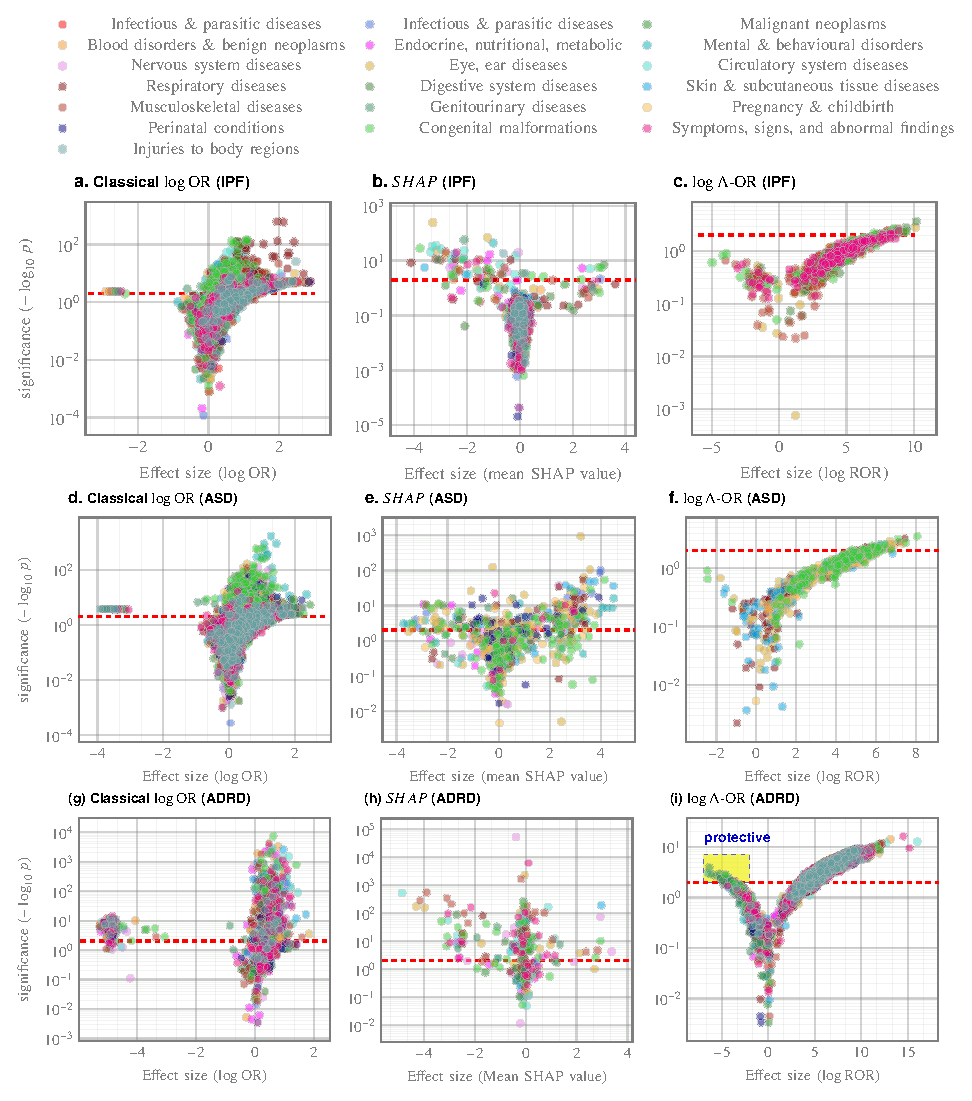
\includegraphics[width=\textwidth]{Figures/External/figvolcano}
  \fi
  
\caption{\textbf{ Comparison of attribution methods (OR, mean SHAP, $\SPOR$) applied to comorbidity profiles for IPF, ASD, and ADRD.} Each point is an ICD code (effect size on x; significance on y). OR and SHAP display pervasive significance and many spuriously ``protective'' codes due to label noise and large-n artifacts; $\SPOR$ collapses this inflated cloud (Theorem~S1), moderating significance and highlighting biologically credible modulators. Data:  Merative Marketscan; $\SPOR$ based on reported \zcor models~\cite{ASDzed,IPFzed,ADRDzed}.  Selection thresholds chosen at 97\% specificity (cases) and 75\% sensitivity.
}\label{figvolcano}
\end{figure} 
%################################### 
%################################### 
%################################### 
%################################### 


%################################### 
%################################### 
%################################### 
%################################### 
%###################################


%==================================================
\section{Application to Large EHR Databases}
%==================================================

$\SPOR$ addresses the principal failure modes of attribution at EHR and biobank scale. It collapses under non-predictive stratification (Theorem~\ref{thm:inherit_collapse} and Corollary~\ref{cor:auc_collapse}), resists amplification of vanishing effects (Lemma~\ref{lem:minimal} together with Corollaries~\ref{corshap} and~\ref{cor:shap_misrank}), and stabilizes correction under explicit label noise via ridge-regularized inversion across plausible $(p,q)$ ranges. The practical upshot is that signals appearing ubiquitous and highly significant under classical OR or SHAP contract markedly when evaluated with $\SPOR$, while biologically credible modulators persist (cf.\ Fig.~\ref{figvolcano}). Intuitively, $\SPOR$ computes exposure odds contrasts across calibrated risk strata and then corrects for outcome misclassification: if the score is uninformative the strata are indistinguishable and the contrast vanishes, whereas true modulators yield consistent separation that survives the correction.

For the analyses below, diagnoses are represented using ICD-10-CM codes recorded in the EHR. In this setting, exposures are defined as binary indicators of recorded ICD diagnosis codes. A code either appears in a patient's record or it does not, so there is no concept of missingness in the conventional sense. Rather, the number of such observations per patient is typically limited, i.e., the data are sparse and potentially noise-corrupted.

Fig.~\ref{figvolcano} and Table~\ref{tabfrac} illustrate the implications of these guarantees. The volcano plots display effect size (log $\SPOR$) against $-\log_{10}(p)$, where $p$ is computed from the Wald statistic using the variance estimator described above. Consequently, the vertical position of each exposure is determined by the estimated uncertainty of the corrected estimator, so the plot directly reflects which associations cross significance thresholds and are prioritized for follow-up investigation. Exposures with large positive $\lambda$-OR values and stable uncertainty correspond to candidate risk factors for the target condition, whereas exposures with negative $\lambda$-OR values that remain significant after correction indicate candidate protective associations, which may be clinically important when modifiable. In contrast, naive odds ratios and SHAP values attribute significance to a wide cloud of diagnostic codes, with a substantial fraction appearing spuriously protective, while $\SPOR$ retains only a narrower set of plausible modulators. Across ASD, IPF, and ADRD, the fraction of codes deemed significant by classical OR or SHAP is reduced several-fold, while the protective codes, often biologically implausible, are almost entirely eliminated.



{\color{red} In these runs, the total number of features (ICD codes) used were as follows: IPF 3279, ASD 1459 and ADRD 11678.}


%% %==================================================
%% \section{Application to Large EHR Databases}
%% %==================================================


%% $\SPOR$ addresses the principal failure modes of attribution at EHR and biobank scale. It collapses under non-predictive stratification (Theorem~\ref{thm:inherit_collapse} and Corollary~\ref{cor:auc_collapse}), resists amplification of vanishing effects (Lemma~\ref{lem:minimal} together with Corollaries~\ref{corshap} and~\ref{cor:shap_misrank}), and stabilizes correction under explicit label noise via ridge-regularized inversion across plausible $(p,q)$ ranges. The practical upshot is that signals appearing ubiquitous and highly significant under classical OR or SHAP contract markedly when evaluated with $\SPOR$, while biologically credible modulators persist (cf.\ Fig.~\ref{figvolcano}). Intuitively, $\SPOR$ computes exposure odds contrasts across calibrated risk strata and then corrects for outcome misclassification: if the score is uninformative the strata are indistinguishable and the contrast vanishes, whereas true modulators yield consistent separation that survives the correction.


%% For the analyses below, diagnoses are represented using ICD-10-CM codes recorded in the EHR. In this setting, exposures are defined as binary indicators of recorded ICD diagnosis codes. A code either appears in a patient's record or it does not, so there is no concept of missingness in the conventional sense. Rather, the number of such observations per patient is typically limited, i.e., the data are sparse and potentially noise-corrupted.


%% Fig.~\ref{figvolcano} and Table~\ref{tabfrac} illustrate the implications of these guarantees. The volcano plots display effect size (log $\SPOR$) against $-\log_{10}(p)$, where $p$ is computed from the Wald statistic using the variance estimator described above; thus the vertical axis is equivalent to ranking associations by the corresponding confidence intervals. Naïve odds ratios and SHAP values attribute significance to a wide cloud of diagnostic codes, with a substantial fraction appearing spuriously “protective,” while $\SPOR$ retains only a narrow set of plausible modulators. Across ASD, IPF, and ADRD, the fraction of codes deemed significant by classical OR or SHAP is reduced several-fold, while the protective codes (often biologically implausible) are almost entirely eliminated.

%% {\color{red} In these runs, the total number of features (ICD codes) used were as follows: IPF 3279, ASD 1459 and ADRD 11678.}



%% In the volcano plots, the vertical position of each exposure is determined by the Wald statistic, which depends on the estimated variance of the $\lambda$-OR estimator. Consequently, the uncertainty of the corrected estimator directly governs which signals cross significance thresholds and are prioritized for follow-up investigation. Exposures with large positive $\lambda$-OR values and stable uncertainty correspond to candidate risk factors for the target condition. Conversely, exposures with negative $\lambda$-OR values that remain significant after correction may indicate potentially protective associations. Identification of such protective exposures may be clinically important, particularly when the exposure is modifiable. Thus the $\lambda$-OR variance provides an uncertainty-aware mechanism for prioritizing signals in large-scale screening analyses.





 %% Fig.~\ref{figvolcano} and Table~\ref{tabfrac}  illustrates the implications of these guarantees:   naïve odds ratios and SHAP values attribute significance to a wide cloud of diagnostic codes, with a substantial fraction appearing spuriously “protective.”, while  $\SPOR$  retains only a narrow set of plausible modulators. Across ASD, IPF, and ADRD, the fraction of codes deemed significant by classical OR or SHAP is reduced several-fold, while the protective codes (often biologically implausible) are almost entirely eliminated.

 For a specific example, $\SPOR$  recovers established ADRD risk domains with strong variance-corrected signals: endocrine or metabolic (hyperparathyroidism, 14.118~\cite{HYPERPARATHYROIDISMmathur2022}; hypo/hyperparathyroidism), sepsis (10.535~\cite{SEPSISzeng2024}), cardio- and cerebrovascular (hypertensive heart and kidney, 9.718~\cite{CKDkelly2022}; hypertension, 6.180~\cite{HYPERTENSIONcarey2023}; atrial fibrillation, 5.511~\cite{ATRIALFIBRpapanastasiou2021}; cerebrovascular, 5.395~\cite{CEREBROVASCULARlove2016}; atherosclerosis, 4.620~\cite{ATHEROSCLEROSISnordestgaard2022}), neurologic/psychiatric (traumatic brain injury, 8.841~\cite{TBIgu2022}; major depressive disorder, 5.432~\cite{DEPRESSIONsaiz2021}; hearing loss, 4.693~\cite{HEARINGlitke2021}; sleep disorders, 2.277~\cite{SLEEPchoe2022}), and metabolic/respiratory/systemic conditions (type 2 diabetes, 4.434~\cite{T2DMathanasaki2022}; COPD, 4.427~\cite{COPDwang2022}; hyperlipidemia, 6.000~\cite{HYPERLIPIDEMIAezkurdia2023}; obesity, 2.791~\cite{OBESITYbeydoun2008}; age-related cataract, 3.930~\cite{CATARACTjun2012}).



The small cluster of apparently ``protective’’ codes lies in reproductive and gynecologic conditions (menstrual irregularities N91–N92, endometriosis N80.9, uterine/breast benign neoplasms D25–D26, cervical findings N84–N88, R87.61, R87.82), consistent with extensive evidence that cumulative estrogen exposure is neuroprotective. Women with longer reproductive spans (later menopause, later age at last childbirth) exhibit reduced dementia risk, whereas abrupt estrogen loss (surgical oophorectomy, premature menopause) is consistently associated with heightened risk. Mechanistically, estrogen supports synaptic and mitochondrial function, reduces $\beta$-amyloid aggregation, buffers oxidative stress, and dampens inflammation, all central to Alzheimer’s pathogenesis~\cite{zarate2017role,Georgakis2016}. Thus, the appearance of these gynecologic codes as “protective’’ is biologically consistent with estrogen-mediated resilience against neurodegeneration.  
A few seemingly unrelated codes also emerged, including attention-deficit hyperactivity disorder (F90), lateral epicondylitis (M77.11), and chronic viral hepatitis C (B18.2),
wherein further investigation is warranted.
 
\subsection*{Concluding remarks}
We have shown that a two–gate selection on a predictive score, combined with a minimal–feasible ridge inversion of the misclassification operator, yields a corrected log-odds ratio with simple Wald inference that removes classical attenuation from non-differential outcome noise. Across controlled simulations, the estimator remains essentially unbiased and sustains markedly higher coverage than the naive alternative over realistic misclassification levels, trading only modest variance. In EHR-scale applications (ADRD, IPF, ASD), it curbs inflated discoveries and spurious “protective” findings seen with naive ORs and model attributions, while surfacing biologically credible modulators. 


\section{Declarations}

\subsection*{Ethics approval and consent to participate}
Not applicable.

\subsection{Consent for publication}
All authors have reviewed and approved the final manuscript and consent to its publication.

\subsection*{Funding}
This work was conducted without support from a specific extramural funding source.

\subsection*{Availability of data and materials}
The analyses rely on existing EHR- and biobank-derived resources accessed under data-use agreements that prohibit public release of individual-level records. De-identified contingency tables sufficient to reproduce all reported figures and tables, together with simulation seeds, will be made available upon publication.

A reference implementation and reproducibility scripts are available at \url{https://doi.org/10.5281/zenodo.17196712} and \url{https://github.com/zeroknowledgediscovery/lambda_or}.

\subsection*{Competing interests}
The authors declare no competing interests.

\subsection*{Authors' contributions}
D.O. analyzed the data and drafted the manuscript. I.C. conceived the study, performed analyses, and co-wrote the manuscript. All authors reviewed and approved the final version.

\subsection*{Acknowledgements}
The authors acknowledge institutional support from the Division of Biomedical Informatics, Department of Internal Medicine, University of Kentucky, and computing resources provided by the University of Kentucky Center for Computational Sciences (CCS; \url{https://www.ccs.uky.edu/}). We thank Robert  Gibbons, Blum-Reise Professor of Medicine
Professor of Public Health Sciences at the University of Chicago, and Dulal Bhaumik,  Professor of Psychiatry, Biostatistics and Bioengineering at the University of Illinois Chicago, for careful reading of an earlier draft and for their constructive feedback.



%% %% BioMed_Central_Bib_Style_v1.01
%% \begin{thebibliography}{27}
%% % BibTex style file: bmc-mathphys.bst (version 2.1), 2014-07-24
%% \ifx \bisbn   \undefined \def \bisbn  #1{ISBN #1}\fi
%% \ifx \binits  \undefined \def \binits#1{#1}\fi
%% \ifx \bauthor  \undefined \def \bauthor#1{#1}\fi
%% \ifx \batitle  \undefined \def \batitle#1{#1}\fi
%% \ifx \bjtitle  \undefined \def \bjtitle#1{#1}\fi
%% \ifx \bvolume  \undefined \def \bvolume#1{\textbf{#1}}\fi
%% \ifx \byear  \undefined \def \byear#1{#1}\fi
%% \ifx \bissue  \undefined \def \bissue#1{#1}\fi
%% \ifx \bfpage  \undefined \def \bfpage#1{#1}\fi
%% \ifx \blpage  \undefined \def \blpage #1{#1}\fi
%% \ifx \burl  \undefined \def \burl#1{\textsf{#1}}\fi
%% \ifx \doiurl  \undefined \def \doiurl#1{\url{https://doi.org/#1}}\fi
%% \ifx \betal  \undefined \def \betal{\textit{et al.}}\fi
%% \ifx \binstitute  \undefined \def \binstitute#1{#1}\fi
%% \ifx \binstitutionaled  \undefined \def \binstitutionaled#1{#1}\fi
%% \ifx \bctitle  \undefined \def \bctitle#1{#1}\fi
%% \ifx \beditor  \undefined \def \beditor#1{#1}\fi
%% \ifx \bpublisher  \undefined \def \bpublisher#1{#1}\fi
%% \ifx \bbtitle  \undefined \def \bbtitle#1{#1}\fi
%% \ifx \bedition  \undefined \def \bedition#1{#1}\fi
%% \ifx \bseriesno  \undefined \def \bseriesno#1{#1}\fi
%% \ifx \blocation  \undefined \def \blocation#1{#1}\fi
%% \ifx \bsertitle  \undefined \def \bsertitle#1{#1}\fi
%% \ifx \bsnm \undefined \def \bsnm#1{#1}\fi
%% \ifx \bsuffix \undefined \def \bsuffix#1{#1}\fi
%% \ifx \bparticle \undefined \def \bparticle#1{#1}\fi
%% \ifx \barticle \undefined \def \barticle#1{#1}\fi
%% \bibcommenthead
%% \ifx \bconfdate \undefined \def \bconfdate #1{#1}\fi
%% \ifx \botherref \undefined \def \botherref #1{#1}\fi
%% \ifx \url \undefined \def \url#1{\textsf{#1}}\fi
%% \ifx \bchapter \undefined \def \bchapter#1{#1}\fi
%% \ifx \bbook \undefined \def \bbook#1{#1}\fi
%% \ifx \bcomment \undefined \def \bcomment#1{#1}\fi
%% \ifx \oauthor \undefined \def \oauthor#1{#1}\fi
%% \ifx \citeauthoryear \undefined \def \citeauthoryear#1{#1}\fi
%% \ifx \endbibitem  \undefined \def \endbibitem {}\fi
%% \ifx \bconflocation  \undefined \def \bconflocation#1{#1}\fi
%% \ifx \arxivurl  \undefined \def \arxivurl#1{\textsf{#1}}\fi
%% \csname PreBibitemsHook\endcsname

%% %%% 1
%% \bibitem[\protect\citeauthoryear{Halpern et~al.}{2016}]{halpern2016electronic}
%% \begin{barticle}
%% \bauthor{\bsnm{Halpern}, \binits{Y.}},
%% \bauthor{\bsnm{Horng}, \binits{S.}},
%% \bauthor{\bsnm{Choi}, \binits{Y.}},
%% \bauthor{\bsnm{Sontag}, \binits{D.}}:
%% \batitle{Electronic medical record phenotyping using the anchor and learn
%%   framework}.
%% \bjtitle{Journal of the American Medical Informatics Association}
%% \bvolume{23}(\bissue{4}),
%% \bfpage{731}--\blpage{740}
%% (\byear{2016})
%% \end{barticle}
%% \endbibitem

%% %%% 2
%% \bibitem[\protect\citeauthoryear{Onishchenko et~al.}{2021}]{ASDzed}
%% \begin{barticle}
%% \bauthor{\bsnm{Onishchenko}, \binits{D.}},
%% \bauthor{\bsnm{Huang}, \binits{Y.}},
%% \bauthor{\bsnm{Horne}, \binits{J.}},
%% \bauthor{\bsnm{Smith}, \binits{P.J.}},
%% \bauthor{\bsnm{Msall}, \binits{M.E.}},
%% \bauthor{\bsnm{Chattopadhyay}, \binits{I.}}:
%% \batitle{Reduced false positives in autism screening via digital biomarkers
%%   inferred from deep comorbidity patterns}.
%% \bjtitle{Science advances}
%% \bvolume{7}(\bissue{41}),
%% \bfpage{0354}
%% (\byear{2021})
%% \end{barticle}
%% \endbibitem

%% %%% 3
%% \bibitem[\protect\citeauthoryear{Onishchenko et~al.}{2022a}]{IPFzed}
%% \begin{barticle}
%% \bauthor{\bsnm{Onishchenko}, \binits{D.}},
%% \bauthor{\bsnm{Marlowe}, \binits{R.J.}},
%% \bauthor{\bsnm{Ngufor}, \binits{C.G.}},
%% \bauthor{\bsnm{Faust}, \binits{L.J.}},
%% \bauthor{\bsnm{Limper}, \binits{A.H.}},
%% \bauthor{\bsnm{Hunninghake}, \binits{G.M.}},
%% \bauthor{\bsnm{Martinez}, \binits{F.J.}},
%% \bauthor{\bsnm{Chattopadhyay}, \binits{I.}}:
%% \batitle{Screening for idiopathic pulmonary fibrosis using comorbidity
%%   signatures in electronic health records}.
%% \bjtitle{Nature Medicine}
%% \bvolume{28}(\bissue{10}),
%% \bfpage{2107}--\blpage{2116}
%% (\byear{2022})
%% \end{barticle}
%% \endbibitem

%% %%% 4
%% \bibitem[\protect\citeauthoryear{Onishchenko et~al.}{2022b}]{JAHAzed}
%% \begin{barticle}
%% \bauthor{\bsnm{Onishchenko}, \binits{D.}},
%% \bauthor{\bsnm{Rubin}, \binits{D.S.}},
%% \bauthor{\bsnm{Horne}, \binits{J.R.}},
%% \bauthor{\bsnm{Ward}, \binits{R.P.}},
%% \bauthor{\bsnm{Chattopadhyay}, \binits{I.}}:
%% \batitle{Cardiac comorbidity risk score: Zero burden machine learning to
%%   improve prediction of postoperative major adverse cardiac events in hip and
%%   knee arthroplasty}.
%% \bjtitle{Journal of the American Heart Association}
%% \bvolume{11}(\bissue{15}),
%% \bfpage{023745}
%% (\byear{2022})
%% \doiurl{10.1161/JAHA.121.023745}
%% \end{barticle}
%% \endbibitem

%% %%% 5
%% \bibitem[\protect\citeauthoryear{Onishchenko et~al.}{2021}]{ADRDzed}
%% \begin{barticle}
%% \bauthor{\bsnm{Onishchenko}, \binits{D.}},
%% \bauthor{\bsnm{Searle}, \binits{S.}},
%% \bauthor{\bsnm{Rockwood}, \binits{K.}},
%% \bauthor{\bsnm{Mastrianni}, \binits{J.}},
%% \bauthor{\bsnm{Chattopadhyay}, \binits{I.}}:
%% \batitle{Rapid universal early screening for alzheimer's disease and related
%%   dementia via pattern discovery in diagnostic history}.
%% \bjtitle{SSRN Electronic Journal}
%% (\byear{2021})
%% \doiurl{10.2139/ssrn.3920640}
%% \end{barticle}
%% \endbibitem

%% %%% 6
%% \bibitem[\protect\citeauthoryear{Choi et~al.}{2016}]{choi2016retain}
%% \begin{botherref}
%% \oauthor{\bsnm{Choi}, \binits{E.}},
%% \oauthor{\bsnm{Bahadori}, \binits{M.T.}},
%% \oauthor{\bsnm{Sun}, \binits{J.}},
%% \oauthor{\bsnm{Kulas}, \binits{J.}},
%% \oauthor{\bsnm{Schuetz}, \binits{A.}},
%% \oauthor{\bsnm{Stewart}, \binits{W.}}:
%% Retain: An interpretable predictive model for healthcare using reverse time
%%   attention mechanism.
%% Advances in neural information processing systems
%% \textbf{29}
%% (2016)
%% \end{botherref}
%% \endbibitem

%% %%% 7
%% \bibitem[\protect\citeauthoryear{GREENLAND}{1996}]{greenland1988sensitivity}
%% \begin{barticle}
%% \bauthor{\bsnm{GREENLAND}, \binits{S.}}:
%% \batitle{Basic methods for sensitivity analysis of biases}.
%% \bjtitle{International Journal of Epidemiology}
%% \bvolume{25}(\bissue{6}),
%% \bfpage{1107}--\blpage{1116}
%% (\byear{1996})
%% \doiurl{10.1093/ije/25.6.1107-a}
%% {\href{https://arxiv.org/abs/https://academic.oup.com/ije/article-pdf/25/6/1107/1957227/25-6-1107.pdf}{{https://academic.oup.com/ije/article-pdf/25/6/1107/1957227/25-6-1107.pdf}}}
%% \end{barticle}
%% \endbibitem

%% %%% 8
%% \bibitem[\protect\citeauthoryear{Lundberg and Lee}{2017}]{lundberg17shap}
%% \begin{bchapter}
%% \bauthor{\bsnm{Lundberg}, \binits{S.M.}},
%% \bauthor{\bsnm{Lee}, \binits{S.-I.}}:
%% \bctitle{A unified approach to interpreting model predictions}.
%% In: \bbtitle{Advances in Neural Information Processing Systems (NeurIPS)},
%% vol. \bseriesno{30},
%% pp. \bfpage{4765}--\blpage{4774}
%% (\byear{2017}).
%% \burl{https://proceedings.neurips.cc/paper/2017/file/8a20a8621978632d76c43dfd28b67767-Paper.pdf}
%% \end{bchapter}
%% \endbibitem

%% %%% 9
%% \bibitem[\protect\citeauthoryear{Slack et~al.}{2020}]{slack2020fooling}
%% \begin{bchapter}
%% \bauthor{\bsnm{Slack}, \binits{D.}},
%% \bauthor{\bsnm{Hilgard}, \binits{S.}},
%% \bauthor{\bsnm{Jia}, \binits{E.}},
%% \bauthor{\bsnm{Singh}, \binits{S.}},
%% \bauthor{\bsnm{Lakkaraju}, \binits{H.}}:
%% \bctitle{Fooling lime and shap: Adversarial attacks on post hoc explanation
%%   methods}.
%% In: \bbtitle{Proceedings of the AAAI/ACM Conference on AI, Ethics, and
%%   Society},
%% pp. \bfpage{180}--\blpage{186}
%% (\byear{2020})
%% \end{bchapter}
%% \endbibitem

%% %%% 10
%% \bibitem[\protect\citeauthoryear{Mathur
%%   et~al.}{2022}]{HYPERPARATHYROIDISMmathur2022}
%% \begin{barticle}
%% \bauthor{\bsnm{Mathur}, \binits{A.}},
%% \bauthor{\bsnm{Ahn}, \binits{J.B.}},
%% \bauthor{\bsnm{Sutton}, \binits{W.}},
%% \bauthor{\bsnm{Chu}, \binits{N.M.}},
%% \bauthor{\bsnm{Gross}, \binits{A.L.}},
%% \bauthor{\bsnm{Segev}, \binits{D.L.}},
%% \bauthor{\bsnm{McAdams-DeMarco}, \binits{M.}}:
%% \batitle{Secondary hyperparathyroidism (ckd-mbd) treatment and the risk of
%%   dementia}.
%% \bjtitle{Nephrology Dialysis Transplantation}
%% \bvolume{37}(\bissue{11}),
%% \bfpage{2111}--\blpage{2118}
%% (\byear{2022})
%% \end{barticle}
%% \endbibitem

%% %%% 11
%% \bibitem[\protect\citeauthoryear{Zeng et~al.}{2024}]{SEPSISzeng2024}
%% \begin{barticle}
%% \bauthor{\bsnm{Zeng}, \binits{Y.}},
%% \bauthor{\bsnm{Cao}, \binits{S.}},
%% \bauthor{\bsnm{Pang}, \binits{K.}},
%% \bauthor{\bsnm{Tang}, \binits{J.}},
%% \bauthor{\bsnm{Lin}, \binits{G.}}:
%% \batitle{Causal association between sepsis and neurodegenerative diseases: a
%%   bidirectional two-sample mendelian randomization study}.
%% \bjtitle{Journal of Alzheimers Disease}
%% \bvolume{97}(\bissue{1}),
%% \bfpage{229}--\blpage{237}
%% (\byear{2024})
%% \end{barticle}
%% \endbibitem

%% %%% 12
%% \bibitem[\protect\citeauthoryear{Kelly and Rothwell}{2022}]{CKDkelly2022}
%% \begin{barticle}
%% \bauthor{\bsnm{Kelly}, \binits{D.M.}},
%% \bauthor{\bsnm{Rothwell}, \binits{P.M.}}:
%% \batitle{Disentangling the relationship between chronic kidney disease and
%%   cognitive disorders}.
%% \bjtitle{Frontiers in neurology}
%% \bvolume{13},
%% \bfpage{830064}
%% (\byear{2022})
%% \end{barticle}
%% \endbibitem

%% %%% 13
%% \bibitem[\protect\citeauthoryear{Carey and
%%   Fossati}{2023}]{HYPERTENSIONcarey2023}
%% \begin{barticle}
%% \bauthor{\bsnm{Carey}, \binits{A.}},
%% \bauthor{\bsnm{Fossati}, \binits{S.}}:
%% \batitle{Hypertension and hyperhomocysteinemia as modifiable risk factors for
%%   alzheimer's disease and dementia: New evidence, potential therapeutic
%%   strategies, and biomarkers}.
%% \bjtitle{Alzheimer's \& Dementia}
%% \bvolume{19}(\bissue{2}),
%% \bfpage{671}--\blpage{695}
%% (\byear{2023})
%% \end{barticle}
%% \endbibitem

%% %%% 14
%% \bibitem[\protect\citeauthoryear{Papanastasiou
%%   et~al.}{2021}]{ATRIALFIBRpapanastasiou2021}
%% \begin{barticle}
%% \bauthor{\bsnm{Papanastasiou}, \binits{C.A.}},
%% \bauthor{\bsnm{Theochari}, \binits{C.A.}},
%% \bauthor{\bsnm{Zareifopoulos}, \binits{N.}},
%% \bauthor{\bsnm{Arfaras-Melainis}, \binits{A.}},
%% \bauthor{\bsnm{Giannakoulas}, \binits{G.}},
%% \bauthor{\bsnm{Karamitsos}, \binits{T.D.}},
%% \bauthor{\bsnm{Palaiodimos}, \binits{L.}},
%% \bauthor{\bsnm{Ntaios}, \binits{G.}},
%% \bauthor{\bsnm{Avgerinos}, \binits{K.I.}},
%% \bauthor{\bsnm{Kapogiannis}, \binits{D.}}, \betal:
%% \batitle{Atrial fibrillation is associated with cognitive impairment, all-cause
%%   dementia, vascular dementia, and alzheimer’s disease: a systematic review
%%   and meta-analysis}.
%% \bjtitle{Journal of general internal medicine}
%% \bvolume{36},
%% \bfpage{3122}--\blpage{3135}
%% (\byear{2021})
%% \end{barticle}
%% \endbibitem

%% %%% 15
%% \bibitem[\protect\citeauthoryear{Love and
%%   Miners}{2016}]{CEREBROVASCULARlove2016}
%% \begin{barticle}
%% \bauthor{\bsnm{Love}, \binits{S.}},
%% \bauthor{\bsnm{Miners}, \binits{J.S.}}:
%% \batitle{Cerebrovascular disease in ageing and alzheimer’s disease}.
%% \bjtitle{Acta neuropathologica}
%% \bvolume{131},
%% \bfpage{645}--\blpage{658}
%% (\byear{2016})
%% \end{barticle}
%% \endbibitem

%% %%% 16
%% \bibitem[\protect\citeauthoryear{Nordestgaard
%%   et~al.}{2022}]{ATHEROSCLEROSISnordestgaard2022}
%% \begin{barticle}
%% \bauthor{\bsnm{Nordestgaard}, \binits{L.T.}},
%% \bauthor{\bsnm{Christoffersen}, \binits{M.}},
%% \bauthor{\bsnm{Frikke-Schmidt}, \binits{R.}}:
%% \batitle{Shared risk factors between dementia and atherosclerotic
%%   cardiovascular disease}.
%% \bjtitle{International Journal of Molecular Sciences}
%% \bvolume{23}(\bissue{17}),
%% \bfpage{9777}
%% (\byear{2022})
%% \end{barticle}
%% \endbibitem

%% %%% 17
%% \bibitem[\protect\citeauthoryear{Gu et~al.}{2022}]{TBIgu2022}
%% \begin{barticle}
%% \bauthor{\bsnm{Gu}, \binits{D.}},
%% \bauthor{\bsnm{Ou}, \binits{S.}},
%% \bauthor{\bsnm{Liu}, \binits{G.}}:
%% \batitle{Traumatic brain injury and risk of dementia and alzheimer’s disease:
%%   a systematic review and meta-analysis}.
%% \bjtitle{Neuroepidemiology}
%% \bvolume{56}(\bissue{1}),
%% \bfpage{4}--\blpage{16}
%% (\byear{2022})
%% \end{barticle}
%% \endbibitem

%% %%% 18
%% \bibitem[\protect\citeauthoryear{S{\'a}iz-V{\'a}zquez
%%   et~al.}{2021}]{DEPRESSIONsaiz2021}
%% \begin{barticle}
%% \bauthor{\bsnm{S{\'a}iz-V{\'a}zquez}, \binits{O.}},
%% \bauthor{\bsnm{Gracia-Garc{\'\i}a}, \binits{P.}},
%% \bauthor{\bsnm{Ubillos-Landa}, \binits{S.}},
%% \bauthor{\bsnm{Puente-Mart{\'\i}nez}, \binits{A.}},
%% \bauthor{\bsnm{Casado-Yusta}, \binits{S.}},
%% \bauthor{\bsnm{Olaya}, \binits{B.}},
%% \bauthor{\bsnm{Santab{\'a}rbara}, \binits{J.}}:
%% \batitle{Depression as a risk factor for alzheimer’s disease: a systematic
%%   review of longitudinal meta-analyses}.
%% \bjtitle{Journal of clinical medicine}
%% \bvolume{10}(\bissue{9}),
%% \bfpage{1809}
%% (\byear{2021})
%% \end{barticle}
%% \endbibitem

%% %%% 19
%% \bibitem[\protect\citeauthoryear{Litke et~al.}{2021}]{HEARINGlitke2021}
%% \begin{barticle}
%% \bauthor{\bsnm{Litke}, \binits{R.}},
%% \bauthor{\bsnm{Garcharna}, \binits{L.C.}},
%% \bauthor{\bsnm{Jiwani}, \binits{S.}},
%% \bauthor{\bsnm{Neugroschl}, \binits{J.}}:
%% \batitle{Modifiable risk factors in alzheimer disease and related dementias: a
%%   review}.
%% \bjtitle{Clinical therapeutics}
%% \bvolume{43}(\bissue{6}),
%% \bfpage{953}--\blpage{965}
%% (\byear{2021})
%% \end{barticle}
%% \endbibitem

%% %%% 20
%% \bibitem[\protect\citeauthoryear{Choe et~al.}{2022}]{SLEEPchoe2022}
%% \begin{barticle}
%% \bauthor{\bsnm{Choe}, \binits{Y.M.}},
%% \bauthor{\bsnm{Suh}, \binits{G.-H.}},
%% \bauthor{\bsnm{Kim}, \binits{J.W.}},
%% \bauthor{\bsnm{Initiative}, \binits{A.D.N.}}, \betal:
%% \batitle{Association of a history of sleep disorder with risk of mild cognitive
%%   impairment and alzheimer’s disease dementia}.
%% \bjtitle{Psychiatry investigation}
%% \bvolume{19}(\bissue{10}),
%% \bfpage{840}
%% (\byear{2022})
%% \end{barticle}
%% \endbibitem

%% %%% 21
%% \bibitem[\protect\citeauthoryear{Athanasaki et~al.}{2022}]{T2DMathanasaki2022}
%% \begin{barticle}
%% \bauthor{\bsnm{Athanasaki}, \binits{A.}},
%% \bauthor{\bsnm{Melanis}, \binits{K.}},
%% \bauthor{\bsnm{Tsantzali}, \binits{I.}},
%% \bauthor{\bsnm{Stefanou}, \binits{M.I.}},
%% \bauthor{\bsnm{Ntymenou}, \binits{S.}},
%% \bauthor{\bsnm{Paraskevas}, \binits{S.G.}},
%% \bauthor{\bsnm{Kalamatianos}, \binits{T.}},
%% \bauthor{\bsnm{Boutati}, \binits{E.}},
%% \bauthor{\bsnm{Lambadiari}, \binits{V.}},
%% \bauthor{\bsnm{Voumvourakis}, \binits{K.I.}}, \betal:
%% \batitle{Type 2 diabetes mellitus as a risk factor for alzheimer’s disease:
%%   Review and meta-analysis}.
%% \bjtitle{Biomedicines}
%% \bvolume{10}(\bissue{4}),
%% \bfpage{778}
%% (\byear{2022})
%% \end{barticle}
%% \endbibitem

%% %%% 22
%% \bibitem[\protect\citeauthoryear{Wang et~al.}{2022}]{COPDwang2022}
%% \begin{barticle}
%% \bauthor{\bsnm{Wang}, \binits{J.}},
%% \bauthor{\bsnm{Li}, \binits{L.}},
%% \bauthor{\bsnm{Zhang}, \binits{Z.}}, \betal:
%% \batitle{Risk of dementia or cognitive impairment in copd patients: A
%%   meta-analysis of cohort studies}.
%% \bjtitle{Frontiers in Aging Neuroscience}
%% \bvolume{14},
%% \bfpage{962562}
%% (\byear{2022})
%% \doiurl{10.3389/fnagi.2022.962562}
%% \end{barticle}
%% \endbibitem

%% %%% 23
%% \bibitem[\protect\citeauthoryear{Ezkurdia
%%   et~al.}{2023}]{HYPERLIPIDEMIAezkurdia2023}
%% \begin{barticle}
%% \bauthor{\bsnm{Ezkurdia}, \binits{A.}},
%% \bauthor{\bsnm{Ram{\'\i}rez}, \binits{M.J.}},
%% \bauthor{\bsnm{Solas}, \binits{M.}}:
%% \batitle{Metabolic syndrome as a risk factor for alzheimer’s disease: a focus
%%   on insulin resistance}.
%% \bjtitle{International journal of molecular sciences}
%% \bvolume{24}(\bissue{5}),
%% \bfpage{4354}
%% (\byear{2023})
%% \end{barticle}
%% \endbibitem

%% %%% 24
%% \bibitem[\protect\citeauthoryear{Beydoun et~al.}{2008}]{OBESITYbeydoun2008}
%% \begin{barticle}
%% \bauthor{\bsnm{Beydoun}, \binits{M.A.}},
%% \bauthor{\bsnm{Beydoun}, \binits{H.}},
%% \bauthor{\bsnm{Wang}, \binits{Y.}}:
%% \batitle{Obesity and central obesity as risk factors for incident dementia and
%%   its subtypes: a systematic review and meta-analysis}.
%% \bjtitle{Obesity reviews}
%% \bvolume{9}(\bissue{3}),
%% \bfpage{204}--\blpage{218}
%% (\byear{2008})
%% \end{barticle}
%% \endbibitem

%% %%% 25
%% \bibitem[\protect\citeauthoryear{Jun et~al.}{2012}]{CATARACTjun2012}
%% \begin{barticle}
%% \bauthor{\bsnm{Jun}, \binits{G.}},
%% \bauthor{\bsnm{Moncaster}, \binits{J.A.}},
%% \bauthor{\bsnm{Koutras}, \binits{C.}},
%% \bauthor{\bsnm{Seshadri}, \binits{S.}},
%% \bauthor{\bsnm{Buros}, \binits{J.}},
%% \bauthor{\bsnm{McKee}, \binits{A.C.}},
%% \bauthor{\bsnm{Levesque}, \binits{G.}},
%% \bauthor{\bsnm{Wolf}, \binits{P.A.}},
%% \bauthor{\bsnm{St.~George-Hyslop}, \binits{P.}},
%% \bauthor{\bsnm{Goldstein}, \binits{L.E.}}, \betal:
%% \batitle{{$\delta$-Catenin is genetically and biologically associated with
%%   cortical cataract and future Alzheimer-related structural and functional
%%   brain changes}}.
%% \bjtitle{PLoS Genetics}
%% \bvolume{8}(\bissue{11}),
%% \bfpage{1003023}
%% (\byear{2012})
%% \doiurl{10.1371/journal.pgen.1003023}
%% \end{barticle}
%% \endbibitem

%% %%% 26
%% \bibitem[\protect\citeauthoryear{Z{\'a}rate et~al.}{2017}]{zarate2017role}
%% \begin{barticle}
%% \bauthor{\bsnm{Z{\'a}rate}, \binits{S.}},
%% \bauthor{\bsnm{Stevnsner}, \binits{T.}},
%% \bauthor{\bsnm{Gredilla}, \binits{R.}}:
%% \batitle{Role of estrogen and other sex hormones in brain aging.
%%   neuroprotection and dna repair}.
%% \bjtitle{Frontiers in aging neuroscience}
%% \bvolume{9},
%% \bfpage{322754}
%% (\byear{2017})
%% \end{barticle}
%% \endbibitem

%% %%% 27
%% \bibitem[\protect\citeauthoryear{Georgakis et~al.}{2016}]{Georgakis2016}
%% \begin{barticle}
%% \bauthor{\bsnm{Georgakis}, \binits{M.K.}},
%% \bauthor{\bsnm{Kalogirou}, \binits{E.I.}},
%% \bauthor{\bsnm{Diamantaras}, \binits{A.A.}},
%% \bauthor{\bsnm{Daskalopoulou}, \binits{S.S.}},
%% \bauthor{\bsnm{Munro}, \binits{C.A.}},
%% \bauthor{\bsnm{Lyketsos}, \binits{C.G.}},
%% \bauthor{\bsnm{Skalkidou}, \binits{A.}},
%% \bauthor{\bsnm{Petridou}, \binits{E.T.}}:
%% \batitle{Age at menopause and duration of reproductive period in association
%%   with dementia and cognitive function: a systematic review and meta-analysis}.
%% \bjtitle{Psychoneuroendocrinology}
%% \bvolume{73},
%% \bfpage{224}--\blpage{243}
%% (\byear{2016})
%% \doiurl{10.1016/j.psyneuen.2016.08.003}
%% \end{barticle}
%% \endbibitem

%% \end{thebibliography}


\bibliographystyle{biometrika}
\bibliography{spor,ad,adrd_risk_factors,zed}

 %======================================================================
% Appendix / Supplementary: Variance derivation for log(SPOR) via delta method
%======================================================================
\appendix
\renewcommand{\thesection}{Appendix \arabic{section}}
\setcounter{section}{0}
\section{Delta-method variance propagation for $\logor^{(\lambda)}$}\label{app:variance}

This appendix derives the additional variance component in $\logor^{(\lambda)}$ arising from estimation of the
selection-conditional misclassification rates $(p_{\mathrm{sel}},q_{\mathrm{sel}})$.

\subsection*{Setup and notation}

Let $\tilde T$ denote the observed $2\times2$ count table on the selected sample ($I=1$),
with entries arranged as
\[
\tilde T=
\begin{bmatrix}
\tilde a & \tilde b\\
\tilde c & \tilde d
\end{bmatrix}.
\]
Let the misclassification operator be
\[
K(p,q)=
\begin{bmatrix}
p & 1-p\\
1-q & q
\end{bmatrix},
\qquad (p,q)=(p_{\mathrm{sel}},q_{\mathrm{sel}}),
\]
so that $K^\top(p,q)$ enters the correction map. For ridge parameter $\lambda\ge 0$, define
\[
A(p,q;\lambda) \equiv (K^\top(p,q)+\lambda I)^{-1},
\qquad
T^{(\lambda)}(p,q) \equiv \tilde T\,A(p,q;\lambda).
\]
Write
\[
T^{(\lambda)}(p,q)=
\begin{bmatrix}
a(p,q) & b(p,q)\\
c(p,q) & d(p,q)
\end{bmatrix},
\]
and define the log-odds functional
\[
\ell(p,q)\equiv \logor^{(\lambda)}(p,q)=\log\frac{a(p,q)\,d(p,q)}{b(p,q)\,c(p,q)}.
\]
All derivatives below are evaluated at the true $(p,q)$.

\subsection*{Differentiating the correction map}

We will use the matrix inverse derivative identity: for an invertible matrix $M(\theta)$,
\[
\frac{\partial}{\partial \theta}M(\theta)^{-1}
=
-\,M(\theta)^{-1}\left(\frac{\partial M(\theta)}{\partial \theta}\right)M(\theta)^{-1}.
\]
Let $M(p,q)=K^\top(p,q)+\lambda I$, so that $A=M^{-1}$.
For $\theta\in\{p,q\}$,
\[
\frac{\partial A}{\partial \theta}
=
-\,A\left(\frac{\partial K^\top}{\partial \theta}\right)A.
\]
Since $T^{(\lambda)}=\tilde T A$,
\[
\frac{\partial T^{(\lambda)}}{\partial \theta}
=
\tilde T \frac{\partial A}{\partial \theta}
=
-\,\tilde T A\left(\frac{\partial K^\top}{\partial \theta}\right)A
=
-\,T^{(\lambda)}\left(\frac{\partial K^\top}{\partial \theta}\right)A.
\]

The required partial derivatives of $K^\top$ are explicit:
\[
\frac{\partial K^\top}{\partial p}
=
\begin{bmatrix}
1 & 0\\
-1 & 0
\end{bmatrix},
\qquad
\frac{\partial K^\top}{\partial q}
=
\begin{bmatrix}
0 & -1\\
0 & 1
\end{bmatrix}.
\]
Thus, letting $T^{(\lambda)}=[t_{ij}]_{i,j\in\{1,2\}}$ and $A=[a_{ij}]_{i,j\in\{1,2\}}$, we obtain
\[
\frac{\partial T^{(\lambda)}}{\partial p}
=
-\,T^{(\lambda)}
\begin{bmatrix}
1 & 0\\
-1 & 0
\end{bmatrix}A,
\qquad
\frac{\partial T^{(\lambda)}}{\partial q}
=
-\,T^{(\lambda)}
\begin{bmatrix}
0 & -1\\
0 & 1
\end{bmatrix}A.
\]

\subsection*{Gradient of the log-odds functional}

Define $g(a,b,c,d)=\log(ad/bc)$. Its partial derivatives are
\[
\frac{\partial g}{\partial a}=\frac{1}{a},\qquad
\frac{\partial g}{\partial b}=-\frac{1}{b},\qquad
\frac{\partial g}{\partial c}=-\frac{1}{c},\qquad
\frac{\partial g}{\partial d}=\frac{1}{d}.
\]
By the chain rule, for $\theta\in\{p,q\}$,
\[
\frac{\partial \ell}{\partial \theta}
=
\frac{1}{a}\frac{\partial a}{\partial \theta}
-\frac{1}{b}\frac{\partial b}{\partial \theta}
-\frac{1}{c}\frac{\partial c}{\partial \theta}
+\frac{1}{d}\frac{\partial d}{\partial \theta},
\]
where $(\partial a/\partial\theta,\partial b/\partial\theta,\partial c/\partial\theta,\partial d/\partial\theta)$
are read off from the matrix $\partial T^{(\lambda)}/\partial\theta$ above.

Equivalently, writing $\mathrm{vec}(\cdot)$ for row-wise vectorization and
\[
u(a,b,c,d)\equiv \left(\frac{1}{a},-\frac{1}{b},-\frac{1}{c},\frac{1}{d}\right)^\top,
\]
we can express the gradient compactly as
\[
\frac{\partial \ell}{\partial \theta}
=
u(a,b,c,d)^\top\,\mathrm{vec}\!\left(\frac{\partial T^{(\lambda)}}{\partial \theta}\right),
\qquad \theta\in\{p,q\}.
\]

\subsection*{Multivariate delta method and variance decomposition}

Let $\hat\theta=(\hat p_{\mathrm{sel}},\hat q_{\mathrm{sel}})^\top$ be obtained from an external validation cohort,
and assume it is independent of the analysis sample used to form $\tilde T$.
A first-order Taylor expansion gives
\[
\ell(\hat\theta)\approx \ell(\theta) + \nabla_\theta \ell(\theta)^\top(\hat\theta-\theta),
\]
hence
\[
\mathrm{Var}(\ell(\hat\theta))
\approx
\mathrm{Var}(\ell(\theta)\mid \theta)
+
\nabla_\theta \ell(\theta)^\top\,\mathrm{Cov}(\hat\theta)\,\nabla_\theta \ell(\theta),
\]
where $\nabla_\theta \ell = (\partial\ell/\partial p,\partial\ell/\partial q)^\top$ and the first term is the
classical large-sample variance for a log-odds ratio computed from the corrected table:
\[
\mathrm{Var}_{\mathrm{naive}}(\ell)\approx \frac{1}{a}+\frac{1}{b}+\frac{1}{c}+\frac{1}{d}.
\]
The second term is the additional variance contribution from estimating $(p_{\mathrm{sel}},q_{\mathrm{sel}})$:
\[
\mathrm{Var}_{\mathrm{extra}}(\ell)
\approx
\nabla_\theta \ell(\theta)^\top\,\mathrm{Cov}(\hat\theta)\,\nabla_\theta \ell(\theta).
\]

\subsection*{Working diagonal approximation for $\mathrm{Cov}(\hat\theta)$}

When $\hat p_{\mathrm{sel}}$ and $\hat q_{\mathrm{sel}}$ are estimated from independent binomial samples in the
validation cohort (e.g., sensitivity estimated among known cases and specificity among known controls),
we use the working approximation $\mathrm{Cov}(\hat p_{\mathrm{sel}},\hat q_{\mathrm{sel}})\approx 0$ and
\[
\mathrm{Var}(\hat p_{\mathrm{sel}})\approx \frac{p_{\mathrm{sel}}(1-p_{\mathrm{sel}})}{n_{\mathrm{val}}},
\qquad
\mathrm{Var}(\hat q_{\mathrm{sel}})\approx \frac{q_{\mathrm{sel}}(1-q_{\mathrm{sel}})}{n_{\mathrm{val}}},
\]
so that
\[
\mathrm{Var}_{\mathrm{extra}}(\ell)
\approx
\left(\frac{\partial \ell}{\partial p_{\mathrm{sel}}}\right)^2 \mathrm{Var}(\hat p_{\mathrm{sel}})
+
\left(\frac{\partial \ell}{\partial q_{\mathrm{sel}}}\right)^2 \mathrm{Var}(\hat q_{\mathrm{sel}}).
\]

\subsection*{Ill-conditioning insight}

Because $\partial A/\partial\theta$ contains the factor $A(\cdot)A$, the gradient magnitude is controlled by
$\|A\|^2=\|(K^\top+\lambda I)^{-1}\|^2$. Thus, as $p_{\mathrm{sel}}+q_{\mathrm{sel}}-1$ approaches $0$ and $K$ becomes
near-singular, the additional variance term can increase sharply, reflecting the instability of the inverse problem.



















\end{document}
